\documentclass[12pt,a4paper]{scrartcl}
\usepackage[utf8x]{inputenc}
\usepackage{ucs}
\usepackage[german]{babel}
\usepackage{textcomp}
\usepackage{graphicx}
\usepackage{wrapfig} %Grafiken von Text umfliessen lassen
\usepackage{multicol} %zweispaltiger Text
\usepackage{multirow} %mehrere Tabellenzeilen zu einer zusammenfassen
\usepackage{rotating} %Rotation von Schrift
\usepackage{wallpaper} %Bilder auch ans Hintergrundbilder einbinden
\usepackage{hyperref} %Um in der PDF-Version klickbare Hyperlinks zu haben
\usepackage{color} % für Farben im allgemeinen
\usepackage{colortbl} %farbige Tabellen
\usepackage[final]{pdfpages}
\usepackage[a4paper,left=15mm,right=15mm, top=12mm, bottom=26mm]{geometry} %Seitenränder
\usepackage{paralist}

%%%%%%%%%%%%%%%%%%%%%%%%%%%%%%%%%%%%%%%%%%%%%%%%%%%%
% Variablen
\newcommand{\emailfachschaft}{\raisebox{-0.5mm}{
\includegraphics{bilder/email_fachschaft}}~}
%\setcounter{tocdepth}{1} % Tiefe des Inhaltsverzeichnisses auf 1(=section) setzen

%%%%%%%%%%%%%%%%%%%%%%%%%%%%%%%%%%%%%%%%%%%%%%%%%%%%
% eigene Kommandos
\newcommand{\spaltenanfang}{\begin{multicols}{2}}
\newcommand{\spaltenende}{\end{multicols}}

\newcounter{mycounter}
\newenvironment{noindEnumerate}
{\begin{list}{\arabic{mycounter}.~~}{\usecounter{mycounter} \labelsep=0pt \labelwidth=0pt \leftmargin=0pt \itemindent=0pt \itemsep=-5pt}}
	{\end{list}}
\newenvironment{noindItemize}
{\begin{list}{\labelitemi}{\usecounter{mycounter} \labelsep=5pt \labelwidth=0pt \leftmargin=5pt \itemindent=0pt \itemsep=-5pt}}
	{\end{list}}


\begin{document}
%%%%%%%%%%%%%%%%%%%%%%%%%%%%%%%%%%%%%%%%%%%%%%%%%%%%
% Titelseite
\begin{titlepage}

\thispagestyle{empty}
\title{\Huge{Don't Panic! 42}}
\author{Magazin für die OE WS 2015}
\date{Herausgegeben von der Fachschaft Informatik}


%\begin{document}

\ThisCenterWallPaper{1.0}{bilder/bender_titelseite4}
\maketitle
\newpage
\end{titlepage}


%%%%%%%%%%%%%%%%%%%%%%%%%%%%%%%%%%%%%%%%%%%%%%%%%%%%
% Inhaltsverzeichnis
\setcounter{tocdepth}{2} %stop at subsections
\tableofcontents
\newpage

%%%%%%%%%%%%%%%%%%%%%%%%%%%%%%%%%%%%%%%%%%%%%%%%%%%%
% Willkommen
\section*{Ei Guude!}
Da seid ihr also. Die Neuen. Und ihr seid hier aus einem Grund. Einem spezifischen Grund. Ihr wollt was lernen.
Und das werdet ihr. An der Uni lernt ihr, so wie wir das gelernt haben,
\"uber jegliche Form der Ahnungslosigkeit hinwegzut\"auschen. Und wir helfen euch dabei!\\
Daher pr\"asentiert die Fachschaft Informatik euch voller Stolz und Selbstverherrlichung die \emph{Don't Panic! 42}.

Und damit fangen wir auch mit der ersten Lektion in Sachen Hochschulkultur an: Selbstbeweihr\"aucherung.
Damit ihr ganz genau wisst, auf wen ihr die Schuld schieben k\"onnt, sind hier alle, die an der Don't Panic! mitgearbeitet haben:
\begin{itemize}
	\item Alexandra Herrmann - Kein Typ
	\item Jonathan Cyriax Brast - Ein Typ
	\item Joshua Sole - Noch ein Typ
	\item Johannes Göpel - Datentyp
	\item Kyle Rinfreschi - Auch ein Typ
	\item Linda Homeier - Typin
	\item Manuel Dittrich - UnTypisch  
	\item Shayan Naderi - orientalischer Typ
	\item Sandra Stelzenmüller - Typendes
	\item Tobias Rothenberger - RBI Typ
	\item \LaTeX - stark typisiert
	\item Und aus historischen Gr\"unden all unsere Vorg\"anger:
	Johannes Sch\"opp, Simon Pruy, Pavel Safre, Grzegorz Lato, Markus Palcer, Tim F\"oller, Sabrina Brandt, Markus Strobel, Michael Bals, Christoph Burschka, Sebastian Behr, Max Hahn-Klimroth und Igor Geier.
\end{itemize}
Außerdem möchten wir Randall Munroe von xkcd (\url{http://xkcd.com}) für die tollen Comics und f\"ur deren Lizenzierung unter Creative Commons (CC) danken.\\

\begin{flushright}Die Fachschaft\\\tiny kollektives Schwarmbewusstsein der Informatik\end{flushright}


%%%%%%%%%%%%%%%%%%%%%%%%%%%%%%%%%%%%%%%%%%%%%%%%%%%%
% Impressum
\section{Impressum}
\spaltenanfang
\noindent\textbf{Studentische Vertretung der Lehreinheit Informatik der Johann Wolfgang Goethe-Universität Frankfurt am Main}\\
Robert-Mayer-Straße 11 - 15\\
D-60325 Frankfurt am Main\\
\url{www.fsinf-frankfurt.de}\\
\url{www.fsinf-forum.de}\\
\emailfachschaft\\
%~\newline
Don‘t Panic! 42\\
OE SoSe 2016\\
Oft überarbeitete und erweiterte Auflage\\
Version der Ausgabe: 2.0\\
April 2016\\
Erscheinungsweise: jedes Semester\\
Auflage: 250\\
Druck und Bindung: HRZ Druckzentrum

\spaltenende

\newpage

%%%%%%%%%%%%%%%%%%%%%%%%%%%%%%%%%%%%%%%%%%%%%%%%%%%%
% Hallo
\section{Hallo erstmal...}
\spaltenanfang
Herzlich willkommen bei uns am Fachbereich! Was du gerade in deinen Händen
hältst, ist die Zeitschrift der diessemestrigen Orientierungsveranstaltung, die
wir „Don’t Panic“ getauft haben. \textbf{Don’t Panic!} - das soll auch als
Motto über der ganzen Veranstaltung stehen. Diesmal nur leicht editiert,
da wir nachdem wir das letzte mal alles in einer Nacht geschrieben haben,
so viele Kommafehler eingebaut hatten, das die \textbf{Don't Panic!} eine Seite
l"anger wurde. 


Naja,jetzt ist erst mal wieder Semesteranfang, und es haben sich lauter Menschen entschlossen,
in Frankfurt einen Studiengang der Informatik aufzunehmen. Darunter sind
Einige, die schon vorher etwas anderes studiert haben oder von einer anderen
Hochschule kommen. Die kennen sich meist schon recht gut im Uni-Dschungel aus,
und auch die ganzen Begriffe, Abkürzungen und Redewendungen sind für sie keine
böhmischen Dörfer mehr. Aber für einen beachtlichen Teil der Erstsemester ist
erfahrungsgemäß so ziemlich alles neu. Und deswegen werden wir uns bemühen,
euch während dieser Orientierungsveranstaltung so ziemlich alles zu erklären.
Ihr werdet hoffentlich schnell merken, dass das alles halb so wild ist und kein
Grund zur Panik besteht, also \textbf{Don’t Panic!} Bei dieser
Orientierungsveranstaltung haben wir uns im Wesentlichen zwei Ziele gesetzt:


Wir wollen euch mit allen notwendigen Informationen versorgen, damit ihr an
eurem ersten Tag in der Uni wenigstens so ungefähr wisst, wo die wichtigsten
Einrichtungen sind, welche Veranstaltungen so laufen und welche davon für euch
Sinn machen. Wir wollen euch ein paar Ratschläge und Tipps mit auf den Weg
geben, und nicht zuletzt können wir euch von einer großen Sammlung von Fehlern
berichten, die wir gemacht haben und die \textsl{ihr} ja nicht unbedingt noch
mal machen müsst.


Das Uni-Leben und das Informatik-Studium bringen viele Begriffe mit sich, die
euch vielleicht unbekannt sind. Vielleicht möchtet ihr einige Stichworte auch
noch einmal in kompakter Form nachlesen. Aus diesem Grund haben wir euch ein
Glossar der wichtigsten Begriffe zusammengestellt.


Aber wir möchten auch, dass ihr euch heute gegenseitig ein
bisschen kennenlernt, damit euch am nächsten Montag wenigstens schon ein paar
Gesichter bekannt vorkommen, wenn der Stress losgeht. Ganz generell empfehlen
wir, sich in kleinen Gruppen zusammenzutun. In einer Gruppe weiß eigentlich
immer jemand, was wo aushängt, bis wann man sich irgendwo eingetragen haben
muss und Vieles mehr. Auch das eigentliche Studieren, das Lernen und das Lösen
von Aufgaben ist in einer Gruppe wesentlich erfolgversprechender und mit
Sicherheit angenehmer.\\
\spaltenende

\newpage

%%%%%%%%%%%%%%%%%%%%%%%%%%%%%%%%%%%%%%%%%%%%%%%%%%%%
% Glossar
\label{glossar}
\section{Deklarative Defintionen der Dinge - Das Dictionary}
In typischer Informatikermanier definieren wir am Anfang, was denn so wichtig sein k\"onnte. Also pr\"asentieren wir euch: Das deklarative W\"orterbuch der bisher eventuell unbenannten Dinge:
\spaltenanfang
\paragraph{AStA -} \glqq Allgemeiner Studierendenausschuss\grqq . Ist so etwas wie die "Regierung" für die Studierendenschaft. Es hört nur niemand drauf. Ist aktuell überwiegend von Sozial- und Rechtswissenschaften dominiert und wird vom $ \rightarrow $StuPa gewählt.  
\paragraph{B.Sc. -}\glqq Bachelor of Science\grqq . Ist der erste Abschluss, den ihr als Informatiker bekommen könnt.
\paragraph{Bachelorordnung -} Das Regelwerk, wie ihr euren Studienabschluss bekommen könnt. Sollte von jedem Studenten in seinem Studium mindestens einmal gelesen werden!!! Sollten dabei Fragen aufkommen, könnt ihr euch an das Prüfungsamt wenden oder an die Fachschaft.
\paragraph{Bockenheim, Campus -} Die Großbaustelle, auf der du dich gerade befindest. Außerdem soll hier demnächst ein Kulturcampus entstehen. Die Informatik soll von vom Campus Bockenheim an den Campus Riedberg umziehen. In exakt 5 Jahren. Seit 1979. Siehe $ \rightarrow $ Umzug.
\paragraph{CP -} \glqq Creditpoints\grqq . Berechnungseinheiten des ECTS(European Credit Point Transfer System), die hochschulübergreifend angerechnet werden können sollten. Dabei gilt: 1 CP $\approx$ 30 Stunden Arbeitsaufwand.
\paragraph{Dekan -} Der Dekan ist ein Professor des Fachbereichs. Er wird vom Fachbereichsrat gewählt und „leitet die Geschäfte des Fachbereichs“ für einen Zeitraum von drei Jahren, d.h. er vertritt den Fachbereich nach außen und führt den Vorsitz im Fachbereichsrat. Er darf viele Entscheidungen auch selbst treffen, für die früher ein Beschluss des \textbf{FBR} notwendig war.
\paragraph{Dekanat -} siehe \textbf{Dekan}, \textbf{Prodekan} und \textbf{Studiendekan}. Daneben wird der Begriff „Dekanat“ für das Sekretariat eines Fachbereichs benutzt, dort wird ein Fachbereich verwaltet.
\paragraph{Direktorium(I-Rat) -} Das Direktorium ist eigentlich der Institutsrat. Anscheinend klang dies zu langweilig, weshalb das Direktorium auch I-Rat genannt wird.
\paragraph{Direktor, geschäftsführender -} Auch GD genannt, leitet das Direktorium. Außerdem repräsentiert er das Institut nach außen.
\paragraph{Direktorat -}  Hierbei handelt es sich um das Pendant zum Dekanat, nur eben auf In\-sti\-tuts\-ebe\-ne. Sämtliche Angelegenheiten der Informatik kann man zunächst im Direktorat der Informatik regeln. Hier könnt ihr auch die \textbf{Bachelorordnung} erhalten.
\paragraph{Evaluierung/Evaluation -} Studierende müssen per Gesetz in die Evaluierung, sprich die Reflexion und Bewertung von Lehrveranstaltungen einbezogen werden. Das ist im Großen und Ganzen auch der einzige Weg, den Studierende haben, um ihre Meinung zu einer Veranstaltung kund zu tun. Die Alternativen wären nicht ernstzunehmende Nörgelei oder die Fachschaft anzusprechen. Dennoch habt ihr dabei eine einigermaßen anonyme Möglichkeit zu Kritik und Lob und die Professoren bekommen tolle Statistiken. Wenn ihr also zur Mitte  oder zum Ende eines Semesters Evaluierungs-Fragebögen bekommt, nehmt sie ernst und beantwortet die Fragen. Selbst wenn ihr eine Veranstaltung abgebrochen habt (gerade dann!), ist es wichtig zu wissen, warum und was besser gemacht werden müsste.
\paragraph{ECTS -} Gilt allgemein als gescheitert, wird aber immer noch angewendet. Siehe $ \rightarrow $Zombie
\paragraph{Fachschaftsraum -} Ist der kleine Raum, der an die Studentlounge anschließt. Hier finden donnerstags ab 18:00 Uhr die Fachschaftstreffen statt.
\paragraph{Fachschaftstreffen -} Das regelmäßige Treffen der Studierendenvertretung in der Informatik. Es findet Donnerstags ab 18:00 Uhr im Fachschaftsraum statt.
\paragraph{FBR -} \glqq Fachbereichsrat\grqq. Der FBR ist ein Gremium, welches über die zentralen Belange des Fachbereichs 12 entscheidet. Die studentischen Vertreter werden dabei direkt gewählt.
\paragraph{Fischerräume -} Die Rechnerräume der Informatik, welche sich hinter dem Magnushörsaal befinden und nur von außen betretbar sind. Einloggen könnt ihr euch mit eurem RBI-Account.
\paragraph{FS/FS-Inf -} Die Fachschaft bzw. die Fachschaft Informatik. Der Begriff „Fachschaft“ wird aber auch in einem wesentlich engeren Sinn für die wenigen Leutchen benutzt, die sich ganz aktiv um die Belange der Studierenden kümmern. Siehe auch den Artikel „Fachschaftsarbeit“ (Seite \pageref{fachschaftsarbeit}).
\paragraph{HiWis -} Hilfswissenschaftler. Das sind eure \textbf{Tutoren} in den Übungen, die studentischen Mitarbeiter in der Bibliothek oder in der RBI. Diesen günstigen Arbeiterschwärmen kann man sich meist schon nach ein paar Semestern anschließen.
\paragraph{Hörsäle -} Die Hörsäle H I - H IV und H 1 - H 16 findet ihr im Hörsaalgebäude.
\paragraph{HRZ-Account -} Jeder Studierende erhält vom \textbf{\underline{H}ochschul\underline{r}echen\underline{z}entrum} einen Account. Durch diesen lassen sich verschiedene Dienste der Uni Frankfurt nutzen. Leider sind die Accountnamen inzwischen pseudonym und schlecht zu merken. Der wichtigste Nutzungsgrund liegt darin, dass ihr über den Zugang die persönlichen Daten eures Studiums verwalten und euch zu Prüfungen anmelden könnt, siehe dazu auch \textbf{QIS-LSF}. Ansonsten braucht ihr ihn für WLAN (an fast allen Unis Deutschlands), eventuell E-Mail, FTP und andere Dinge. Die Zugangsdaten erhaltet ihr zusammen mit dem \textbf{Studentenausweis}. Nicht zu verwechseln mit dem \textbf{RBI-Account}.
\paragraph{Institutsrat -} Der Institutsrat ist ein Gremium, das die Belange des Institutes Informatik behandelt und teilweise, wo nicht der Fachbereichsrat gefragt ist, entscheidet.
\paragraph{Kommilitonen -} Sind die Leute links und rechts neben dir.
\paragraph{Lernzentrum -}  Befindet sich im Erdgeschoss des Informatikgebäudes, gleich links wenn ihr zum Haupteingang hineinkommt. Hier könnt ihr versuchen zu lernen, sollte ihr euch wider Erwarten doch inmitten von Diskussionen konzentrieren können. Im Lernzentrum sind die Skripte der momentan laufenden Basismodule vorhanden. Außerdem habt ihr hier die Möglichkeit, einen Mitarbeiter der Uni um Hilfe bei euren Aufgaben zu bitten. Es gibt sogar Brettspiele zum Ausleihen. An das Lernzentrum sind die ''Student-Lounge'' genannten Räume der Fachschaft angeschlossen.
\paragraph{Magnus-Hörsaal -} Ist der einzige Hörsaal, den die Informatik im Gebäude hat. Ein echter Klassiker.
\paragraph{Modul -} Ein Modul ist eine Lehreinheit, die fachlich sinnvoll aus ein bis mehreren Lehrveranstaltungen zusammengesetzt ist. Ein Modul wird innerhalb eines Semesters oder auch über 2 Semester veranstaltet.
\paragraph{M.Sc. -} \glqq Master of Science\grqq . Großer Bruder vom Bachelor.
\paragraph{Munchkin -} Ein sehr beliebtes Kartenspiel im Fachbereich. 
\paragraph{Prodekan -} Sowas wie ein stellvertretender Dekan. Der Dekan und der Prodekan können auch eine Art „Aufgabenteilung“ unter sich vereinbaren.
\paragraph{Prüfungsamt -} Im Prüfungsamt meldet man sich für Klausuren, mündliche Prüfungen und Studienleistungen aller Art an. Zwar geschehen inzwischen die meisten Anmeldungen über das \textbf{QIS-LFS}, aber das ist manchmal unzuverlässig.
\paragraph{Prüfungsausschuss -} Der Prüfungsausschuss ist ein Ausschuss der sich mit Prüfungen befasst (Sach bloß!). Hier sitzen Professoren und Studenten, die Entscheidungen treffen, die das \textbf{Prüfungsamt} nicht treffen darf.  Vor allem kann man hier Ausnahmeregelungen formlos beantragen. Dazu schreibt man einfach einen Brief an den Ausschuss, in dem man kurz sagt, was man will, und wieso. Den kann man dann im \textbf{Prüfungsamt} einwerfen.
\paragraph{Prüfungsprotokoll-Datenbanken -} Etwas, bei dem dir ruhig mulmig zu Mute sein darf, ist eine mündliche Prüfung. Doch dem mulmigen Gefühl kann abgeholfen werden: Schau dir doch einfach mal an, was den anderen so passiert ist, als sie in ihrer Prüfung waren. Dafür gibt es eine eigene Datenbank, die ihr unter \url{http://myexam.gdv.cs.uni-frankfurt.de/} finden könnt. Mitmachen ist dabei Pflicht, denn ohne Geben gibt es bei dieser Idee auch kein Nehmen!
\paragraph{QIS-LSF -} Das elektronische Informationssystem der Uni. Hier könnt ihr euch für Prüfungen anmelden, eure Kontaktdaten ändern oder euch den Vorlesungskatalog anschauen. Für das QIS-LSF braucht ihr euren HRZ-Account
\paragraph{Rekursion -} Rekursion - siehe Rekursion!
\paragraph{RBI -} \glqq Rechner-Betriebsgruppe Informatik\grqq . Die RBI kümmert sich um alles, was mit Elektronik in der Informatik zu tun hat. Über euren RBI-Account, den ihr in der RBI beantragen könnt, habt ihr pro Semester 500 Druckseiten frei und könnt noch weitere Angebote nutzen.
\paragraph{Skript -} Entweder eine frühere Mitschrift eines fleißigen Studenten (eher selten anzutreffen) oder die Kopien der vom Professor benutzten Folien, gelegentlich auch ein extra hierfür entworfener Text. Ist entweder in der entsprechenden Fachbereichs-Bibliothek, auf der Internet-Präsenz des jeweiligen Dozenten oder gar nicht zu finden. Dabei sollte man jedoch zwei Dinge beachten: 1. Das Lesen des Skriptes ersetzt nur sehr selten die Teilnahme an der Veranstaltung. 2. Wer ein komplettes Skript auf dem Drucker im RBI ausdruckt, läuft Gefahr, von vor dem Drucker wartenden Kommilitonen gesteinigt zu werden, oder zumindest als DAU (Dümmster anzunehmender User) des Monats nominiert zu werden; vgl. \textbf{RBI}.
\paragraph{Statusgruppen -} Die Statusgruppen der Universität sind Professoren, Studierende, Wissenschaftliche Mitarbeiter (WiMi) und die administrativ-technischen Mitarbeiter (SoMis).
\paragraph{Studentenausweis (Goethe-Card) -} Diese kleine Plastikkarte erfüllt gleich mehrere Aufgaben: sie dient euch als Studierendenausweis, Bibliotheksausweis und als Semesterticket. Der Zeitraum, für den die Goethe-Card gültig ist, wird mit Spezialtinte auf die Karte aufgedruckt. Nach der Rückmeldung könnt ihr den Aufdruck erneuern, indem ihr einen der dafür vorgesehenen Automaten verwendet (z.B. im Gebäude \textit{Neue Mensa}). Durch den enthaltenen Chip werden Informationen zu den von euch ausgeliehenen Büchern gespeichert, außerdem könnt ihr sie als Schlüssel für Schließfächer verwenden. Ihr könnt die Goethe-Card mit Geld ``aufladen'', und mit diesem Guthaben die von der Uni aufgestellten Kopierer nutzen, oder in der Mensa bezahlen.
\paragraph{Studentlounge -} Die \textbf{Fachschaftsräume} hinter dem Lernzentrum, die normalerweise offen sind und von allen Studierenden als eine Erweiterung vom \textbf{Lernzentrum} oder auch als ein Platz, wo man sich auf Sofas entspannen kann, betrachtet werden kann. Auch hier solltet ihr allgemeine Regeln des sozialen Zusammenlebens beachten. Also haltet den Raum sauber, entsorgt euren Müll und haltet euch an die Hausordnung.
\paragraph{Studiendekan -} Auch ein Mitglied der „Drei Dekane“. Er ist im Besonderen zuständig für Fragen von Lehre und Studium.
\paragraph{Studien-Service-Center -} Befindet sich im PEG-Gebäude auf dem Campus Westend. Hier könnt ihr alle Arten von Anträgen(Teilzeit,etc.) stellen.
\paragraph{StuPa -} Das StuPa ist, wie der Name „Studentenparlament“ ja auch sagt, das Parlament der Studierenden. Und wie es sich für jedes ordentliche Parlament gehört, wird auch im StuPa Politik gemacht: Deshalb hält man die StuPa-Sitzungen auch kaum aus. Welche politischen Hochschulgruppen in das StuPa gewählt werden, könnt ihr versuchen in Wahlen zu beeinflussen.
\paragraph{SWS -} Abkürzung für Semesterwochenstunde, sprich die Zeit, die eine Veranstaltung im Verlauf des Semesters wöchentlich dauert. Die private Vor- bzw. Nacharbeit dauert normalerweise noch das doppelte dazu. Also: 1 SWS = 3 Stunden fürs Studium wöchentlich.
\paragraph{Tutor -} Als Tutor endet man aus drei verschiedenen Gründen. Ein Grund wäre, dass ihr CP für euer Ergänzungsmodul braucht und euch dadurch entschieden habt, Tutor zu werden. Der zweite Grund wäre, dass ihr Geld braucht und für einen Studentlohn von 8,50 Euro arbeiten wollt. Oder aber ihr wollt euer Wissen weiter geben bzw. euer Wissen auffrischen. Eine Mischung aus den drei Gründen tritt auch gelegentlich auf.
\paragraph{Umzug -} Eine sehr beliebte Sage innerhalb des Fachbereichs 12. Von Generation zu Generation wird weiter verbreitet, dass wir zum Riedberg umziehen werden. Erste historische Erwähnung dieser Sage wurde in den Protokollen der 4. Ratssitzung des Direktorium für Informatik im Jahre 1979 gefunden.
\paragraph{Variable, metasyntaktisch -} Platzhalter und genereller Ausdruck der Faulheit von Informatikern. Erlaubt einem sich unpr\"azise auszudr\"ucken. Beispielsweise seien hier foo, bar, foobar, xyzzy, Ding, Dinge und Zeuch genannt. Zeuch nimmt dabei eine Sonderstellung ein, da dadurch gerne komplette Prozeduren, Programmbl\"ocke und Krempel von Dingen die Zeuch machen beschrieben wird.
\paragraph{Wahlen -} Irgendwann werdet ihr ein Brief nach Hause bekommen, womit ihr z.B. den FBR oder das StuPa wählen könnt. Damit könnt ihr uns als Fachschaft w\"ahlen oder halt eine neue. Wie ihr wollt. Zum StuPa kommt meistens vor den Wahlen eine Wahlzeitung, in der sich die Gruppen vorstellen.
\paragraph{Wert, metasyntaktisch} Wenn einem nichts einf\"allt nimmt man die. Metasyntaktische Werte haben oft eine besondere Bedeutung, die aber mit der Zeit in Vergessenheit geraten ist. Beispiele sind 7, 42, 37, 0815, 1337, 31337, \texttt{0xdeadbeef}, \texttt{0xcafebabe} und f\"ur Stringkonstanten ''foo''. Werden fast immer \textit{metasyntaktischen Variablen} zugeordnet.
\paragraph{Westend, Campus -} Angeblich der schönste Campus Europas. Und das ist genau da, wo wir nicht sind. Dafür sind da die Geistes-, Gesellschafts- und Sprachwissenschaften sowie die Religionen zu finden. Zu erreichen per Bus mit Linie 36 oder 75, per U-Bahn 1,2,3 oder 8 (Holzhausenstraße) oder falls man Zeit hat auch zu Fuß durch den Palmengarten.
\paragraph{WiMis -} Wissenschaftliche Mitarbeiter. Sie sind an einer Professur angestellt, um dort zu promovieren, also um irgendwann einmal einen Doktortitel zu erhalten. Bis dahin forschen sie fleißig und unterstützen den Professor bei Lehrveranstaltungen. Gerade in Übungen werdet ihr ab und zu mit einem WiMi zu tun haben.
\paragraph{Zombie -} Siehe $ \rightarrow$ECTS
\spaltenende

\begin{center}
	
\includegraphics[scale=0.5]{comics/dictionary-attack}
\end{center}

%%%%%%%%%%%%%%%%%%%%%%%%%%%%%%%%%%%%%%%%%%%%%%%%%%%%
% Studium
\section{Euer Studium}
%%%%%%%%%%%%%%%%%%%%%%%%%%%%%%%%%%%%%%%%%%%%%%%%%%%%
% Stundenplan
\subsection{Ein Stundenplan zum Ausfüllen}
\newcommand{\x}{\parbox[0pt][2.7cm][c]{3.7cm}{\hspace{3.7cm}} }
\newcommand{\xT}{\parbox[0pt][1.6cm][c]{1.9cm}{\hspace{3.7cm}} }
% --- Farbdefinitionen ----------------------------------------
\definecolor{hellgrau}{rgb}{0.95,0.95,0.95}

%\begin{sidewaystable}
%\begin{addmargin}[-2mm]{0cm}

%\begin{center}
%\begin{tabular}{|c|c|c|c|c|c|}
%\hline Zeit & Montag & Dienstag & Mittwoch & Donnerstag & Freitag \\
%\hline 8-10  & \x & \x & \x & \x & \x \\
%\hline 10-12 & \x & \x & \x & \x & \x \\
%\hline 12-14 & \x & \x & \x & \x & \x \\
%\hline 14-16 & \x & \x & \x & \x & \x \\
%\hline 16-18 & \x & \x & \x & \footnotesize 16:00 : Fachschaftstreffen & \x \\
%\hline ab 18 & \x & \x & \x & \x & \x \\
%\hline
%\end{tabular}
%\end{center}

%\end{addmargin}
%\end{sidewaystable}

\vspace{23.6cm} % ein Korrekturabstand wg. Drehen
\begin{center}
\begin{rotate}{90}
\begin{tabular}{|c|c|c|c|c|c|}
\hline \cellcolor{black} \xT
	& \cellcolor{black} \textcolor{white}{\textbf{Montag}}
	& \cellcolor{black} \textcolor{white}{\textbf{Dienstag}}
	& \cellcolor{black} \textcolor{white}{\textbf{Mittwoch}}
	& \cellcolor{black} \textcolor{white}{\textbf{Donnerstag}}
	& \cellcolor{black} \textcolor{white}{\textbf{Freitag}} \\
\hline 8:00-10:00  & \x & \x & \x & \x & \x \\
\hline  \cellcolor{hellgrau}10:00-12:00 &  \cellcolor{hellgrau} \x &  \cellcolor{hellgrau} \x &  \cellcolor{hellgrau} \x &  \cellcolor{hellgrau} \x &  \cellcolor{hellgrau} \x \\
\hline 12:00-14:00 & \x & \x & \x & \x & \x \\
\hline  \cellcolor{hellgrau} 14:00-16:00 &  \cellcolor{hellgrau} \x &  \cellcolor{hellgrau} \x &  \cellcolor{hellgrau} \x &  \cellcolor{hellgrau} \x &  \cellcolor{hellgrau} \x \\
\hline 16:00-18:00 & \x & \x & \x & \footnotesize & \x \\
\hline  \cellcolor{hellgrau} 18:00-20:00 &  \cellcolor{hellgrau} \x &  \cellcolor{hellgrau} \x &  \cellcolor{hellgrau} \x &  \cellcolor{hellgrau} \x &  \cellcolor{hellgrau} \x \\
\hline
\end{tabular}
\end{rotate}
\end{center}

\subsection{Der Bachelor Informatik}
\subsubsection{Studienverlaufsplan}
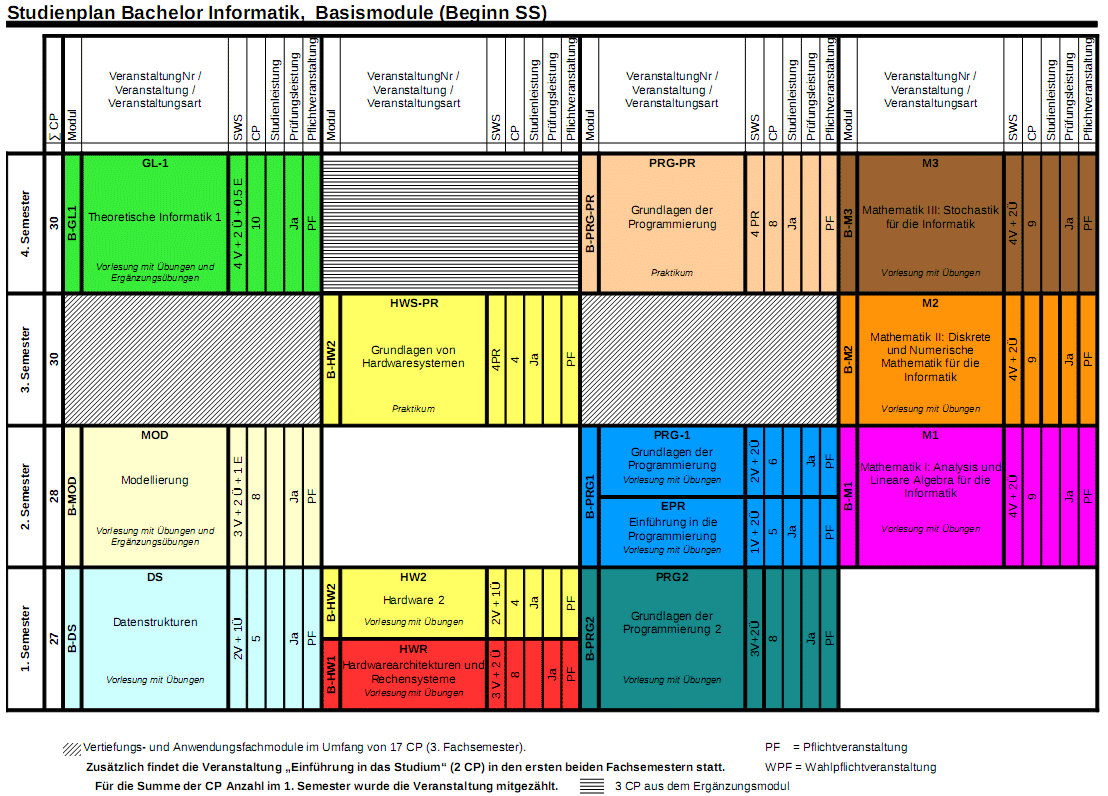
\includegraphics[width=18cm]{bilder/basismodulebachelorSS}
\newline
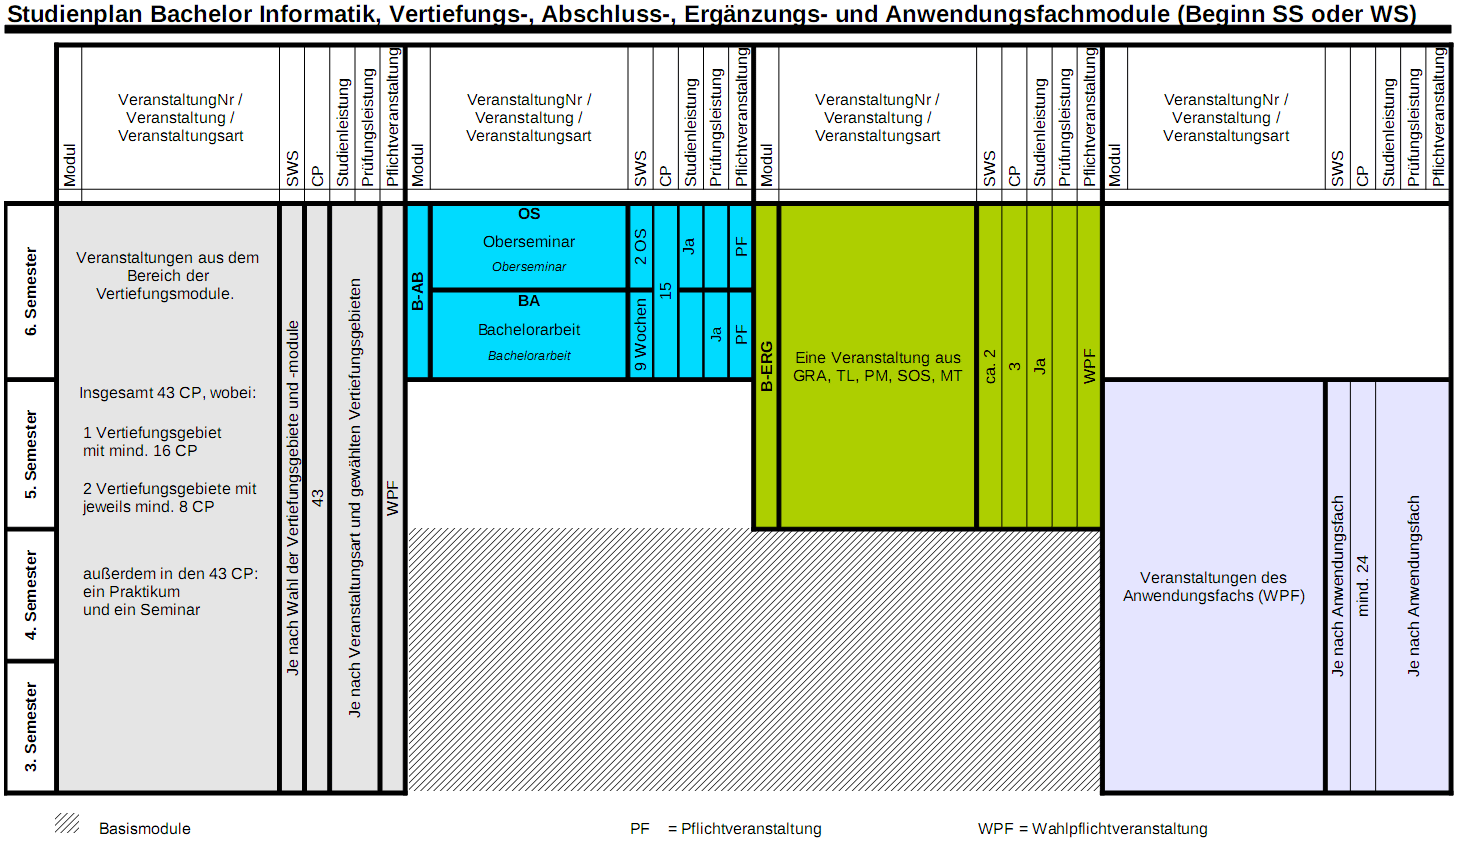
\includegraphics[width=18cm]{bilder/sonstigemodulebachelor}
\newpage
%%%%%%%%%%%%%%%%%%%%%%%%%%%%%%%%%%%%%%%%%%%%%%%%%%%%
% Bachelor Rollenspiel
\subsubsection{Der Bachelor - Ein verkorkstes Rollenspiel}
\spaltenanfang
Was ist eingendlich so ein Bachelor? Denn mein Englisch-Deutsch-W\"orterbuch
sagt, dass ich mich in einen Studiengang eingetragen habe, in dem ich zum
''Jungesellen der Rechner-Wissenschaft'' gemacht werden soll. Und der
Jungesellenstatus in der Wissenschaft kann nicht wirklich mein Ziel sein, oder?

Wie immer: Don't Panic! Bachelor ist nur ein Name, den die Politik \"ubernommen
hat, um internationaler zu klingen.  So ist das halt bei Hochschulreformen. Und
au{\ss}erdem ist was der Bachelor genau ist erst wichtig wenn ihr fertig seit.
Jetzt ist ersmal wichtig dass ihr sinnvoll studieren k\"onnt. Und dazu solltet
ihr ein paar Grundlagen wissen.

\textbf{Merke: Das Bachelorstudium ist im Prinzip ein verkorkstes Rollenspiel}

Als erstes gibt es f\"ur Rollenspielfanatiker und Munchkins das offizielle
Regelwerk zum Studium: Die \textsc{\textit{Bachelorordnung}}. Die besteht wie jedes
Regelwerk aus einem kleinen Teil mit Regeln
%TODO:*U NO SAY*
und dem Teil mit den riesigen
Tabellen, die Zeuch beschreiben. Aber anstatt coole R\"ustung und so gibt es
nur Skills. Nur hei{\ss}en die hier Module und man bekommt die erst, wenn man sie
verdient hat.

Ausserdem gibt es sowas wie XP. Die heissen hier aber CP, weil das alles
bitterer Ernst ist und sich deshalb nicht an g\"angige Rollenspiel
Designkonventionen gehalten wird. Und von denen bekommt man etwa einen pro 30
Stunden Studium.

Aber auch das funktioniert irgendwie anders als man das gewohnt ist. Statt dass
man XP bekommt, mit denen man sich bessere Skills holt um dann in Proben
bessere Chancen zu haben, muss man hier erst die Pr\"ufungen bestehen, bekommt
dann das Modul und damit die CP.
%TODO: *DAFU?*.

{\large
\begin{verbatim}
[XP] -> [skills] -> [pruefungen]
[CP] <- [module] <- [pruefungen]
\end{verbatim}}

\textbf{Bacheloraufbau:}
Schauen wir uns also das System mal genauer an.
Das Ziel ist es den Abschluss Bachelor zu bekommen. Dazu muss man 180CP
bekommen haben, die man mit dem Abschluss von Modulen bekommen hat. Und wie
jeder weiss, muss ein guter Munchkin Min-Maxen. Aber auch das kann der Bachelor
nicht gut.

Um Module abzuschlie\ss en muss man eine Klausur schreiben, eine m\"undliche
Pr\"ufung machen, einen Vortrag halten, gen\"ugend Abgaben gemacht haben, oder
sonst irgendwie gezeigt haben, dass man die CP auch wirklich verdient hat.


\textbf{Die Modulkategorien:}
Die Module sind wie f\"ur Skills \"ublich in verschiedene Kategorien
eingeteilt. Das kann euch sowohl einschr\"anken als auch Freiheiten geben.
Als erstes sind f\"ur euch die \emph{Basismodule} interessant, denn die m\"usst ihr als Informatiker alle machen.\\
Dann kommen die \emph{Vertiefungsmodule} ins Spiel. Hier kann man seinen Studenten in mindestens drei von f\"unf Kategorien spezialisieren.\\
Die \emph{Anwendungsfachmodule} sind Multiklassenskills, in denen ihr Fertigkeiten aus anderen F\"achern lernen sollt.\\
\emph{Erg\"anzungsmodule} sind durch die \texttt{Gute Idee\texttrademark} entstanden, dass Informatiker mindestens 150 Stunden Soft Skills oder soziales Zeuch gemacht haben sollten. Wir wollen doch keine verschrobenen antisozialen Studenten bauen.\\
Und zum Abschluss gibt es das \emph{Abschlussmodul}, das die Bachelorarbeit und das Oberseminar \"uber die Arbeiten enth\"alt.\\

\begin{center}
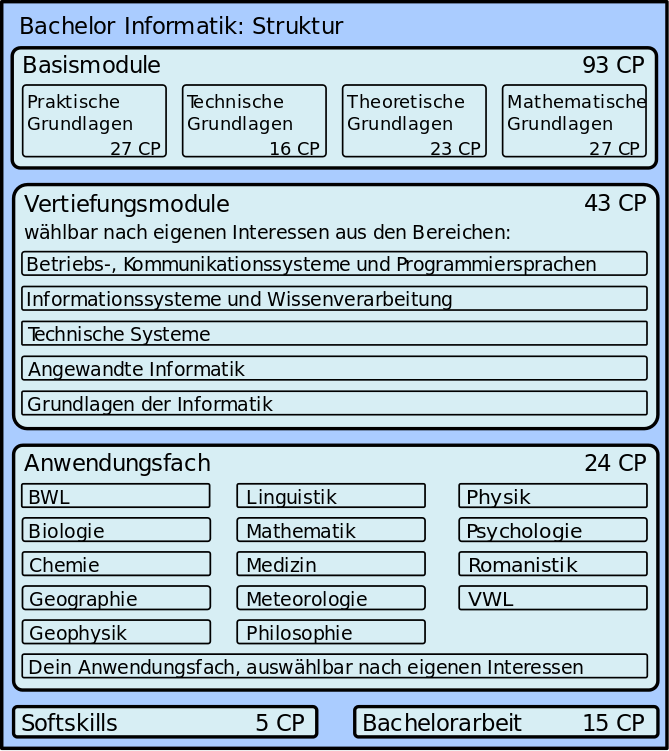
\includegraphics[width=85mm]{bilder/BacInfStruktur}
\end{center}


\textbf{Basismodule:}
Es gibt ein paar Skills die jeder Informatiker haben sollte. Und es gibt
Basismodule. In den Basismodulen lernt ihr offiziell vier Dinge: Mathe, Wie
Computer funktionieren (wird gerne auch ''Hardware'' genannt), Wie man Computer
programmiert und Theoretische Informatik. Das sind alles Vorlesungen, bis auf
das Programmier-Praktikum und das Hardware-Praktikum, die Praktika sind.
Insgesamt gibt es hier 93CP zu holen.

\textbf{Vertiefungsmodule:}
Die gibt es in f\"unf Spezialisierungen: BKSPP, ISWV, TS, ANI und GDI. \emph{''Betriebs-
und Kommunikationssysteme und Progammiersprachen und -paradigmen''} enth\"alt
genau was im Titel steht. \emph{''Informationssysteme und Wissensverarbeitung''}
besch\"aftigt sich mit Textverarbeitung , Datenbanken und k\"unstlicher
Intelligenz. In \emph{''Technische Systeme''} lernt man mehr \"uber Microcontroller,
Rechnerarchitektur und Chipdesign. \emph{''Angewandte Informatik''} ist alles was
sonst nicht untergebracht werden konnte. Da sind dann so Sachen wie
Computergrafik, Zeug und Krempel drin. Wer aber statt Zeug und Krempel lieber
was abgehobenes macht kann in \emph{''Grundlagen der Informatik''} fast schon ein
Mathestudium simulieren. Dort ist mehr Logik, mehr Algorithmentheorie und mehr
Beweise.

Und jetzt kommt der Haken: Du musst mindestens 43CP machen und davon in einem
mindestens 16CP und in zwei anderen mindestens 8CP und die anderen 11CP kannst
du machen wie du willst. Dabei musst du die drei Vertiefungsgebiete, in denen
du leveln willst, dem Pr\"ufungsamt vor der ersten Klausur mitteilen. Alles
Klar? OK!

\textbf{Anwendungsfachmodule:}
Die Muliklassenskills auch Anwendungsfachmodule genannt erlauben euch was anderes als Informatik zu lernen.
Die mei{\ss}ten dieser Nebenfachmodule sind geregelt. Das hei{\ss}t das
Basisregelwerk ''Die Bachelorordnung'' hat vorgefertigte L\"osungen wie ihr das
Nebenfach machen k\"onnt. Ist euer Nebenfach nicht drin, k\"onnt ihr das trotzdem studieren, aber dann halt ungeregelt.
Dazu muss unser Pr\"ufungsamt mit dem ''gegnerischen'' Pr\"ufungsamt ''kl\"aren'' wie das ganze abgewickelt werden soll.
Fakt ist aber, ihr braucht immer mindestens 24CP.

\textbf{Erg\"anzungsmodule:}
Irgendein schlauer Informatiker hat sich mal gedacht: \emph{Wir wollen, das
Frankfurter Informatiker nicht nur Fachidioten sind, sondern auch ''sozial''
sein k\"onnen. Die haben dann ''Soft Skills''. Wie ''Teamf\"ahigkeit'' und so. Und das
ist dann gut.} Aber da zu viel Soziales nicht in den Studienverlausplan passt, macht ihr 5CP.
Da ist dann auch die Studienorientierung STO drin. Die im ersten Semester 2CP gibt, und sp\"ater nur noch halb so viel.
Da wird euch nochmal wie man studiert auf dem Silbertablett gereicht.

\textbf{Die restlichen 15CP:}
Gibt es mit der Bachlorarbeit.

\textbf{Die Bachelorarbeit:}
Das ist sowas wie eine echte wissenschaftliche Arbeit. Wenn ihr die gamcht habt gibt das 15CP im Abschlussmodul.

\begin{center}
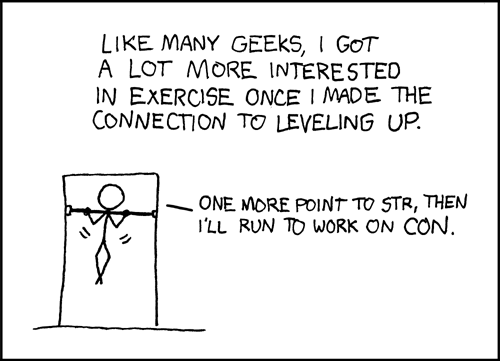
\includegraphics[width=\linewidth]{comics/exercise}\\
\end{center}

\textbf{Die Klausurregeln:}
Und nun steigt die Spannung. Die Klausurphase beginnt.
W\"ahrend im Semester Wochen vergehen k\"onnen, ohne das viel passiert, ist die Klausurphase eher wie Kampfrunden.
Eine Megasekunde, die im echten Leben vergehet, kommt einem wie eine Gigasekunde an der Uni vor.
    Aber keine Panik, es gibt einige Tricks und ein paar Regeln, die ihr
anwenden k\"onnt, um sinnvoll lebendig, und mit ein paar mehr CP durch die
Klausurphase zu kommen.

\textbf{Anmeldung:}
Zu Klausuren m\"usst ihr euch zwei Wochen vorher angemeldet haben. Und vor der ersten Klausur m\"usst ihr euch f\"ur den Bachlor anmelden.
Wenn ihr die Klausur schreibt und nicht angemeldet seit, gibt das keine XCP

\textbf{Timing:}
Zuerst ist wichtig zu planen wann ihr Klausuren schreibt.
Die Termine selbst k\"onnt ihr zwar nicht \"andern, aber ein guter Munchkin hat die Bachelorordnung gelesen
und hat festgestellt, dass viele Klausuren jedes Semester angeboten werden.

Aber wie soll es mir helfen die Klausur zu verschieben?
N\"achstes Semsester sind doch wieder Klausuren, oder?

Aber da ist es wichtig
zu wissen, wie die Professoren diese Regel mit jedem Semester auslegen.
Professoren waren alle mal Studenten und sind deshalb fast so faul wie wir.
Und fast immer m\"ussen Nachklausuren angeboten werden, f\"ur Studenten, die durchgefallen sind oder nicht teilnehmen konnten.
W\"ahrend die Vorlesungen meisstens in der dritten April- oder Oktoberwoche anfangen f\"angt das Semester p\"unklich am Ersten an.

Und deshalb sind die Nachklausuren mei{\ss}tens am Ende der Semesterferien, aber im neuen Semester. Der
ge\"ubte Munchkin braucht also seine Klausuren nicht alle auf einmal zu
schreiben, sondern lernt am Anfang \emph{und} am Ende der Semesterferien.
Ansonsten gilt: \textbf{Konzentrier dich auf wenige Klausuren, statt in allen zu versagen.}
\emph{Bla, bla, lernt rechtzeitig, bla\dots}\\

\textbf{Freiversuche - Rerolls f\"ur Klausuren:}
Und jetzt kommen die kleinen Feinheiten des Regelwerks die jeden Munchkin interessieren sollten.
Ger\"uchteweise haben manche Studenten Klausuren mitgeschrieben und kl\"aglich versagt. Daran ist noch nichts besonderes.
Aber die f\"ur diese Studenten war es so als h\"atten sie die Klausur nie
geschrieben und haben sich einfach beim n\"achsten mal wieder in die Klausur
gesetzt. Und noch viel besser. Andere die grad so bestanden hatten, sa{\ss}en
in der Klausur und konnnten nochmal mitschreiben und haben am Ende eine bessere
Note gehabt. Wie geht das?

Naja, eigendlich ist nichts besonderes daran. Wenn du innerhalb der
Freiversuchsfrist eine Klausur schreibst, kannst du beim ersten Mal
Durchfallen, ohne dass das als Fehlversuch gez\"ahlt wird.
Die Freiversuchsfrist ist in der Bachelorordnung festgelegt und ist an den Studienverlauf angepasst.
Das soll euch dazu motivieren die Klausur zu beim erstem Mal oder in der Nachklausur mitzuschreiben.
Das funktioniert aber nur in den Basismodulen so. In den Vertiefungs und Anwendungsfachmodulen funktioniert das leider nicht.
Aber die Basismodule machen \"uber die H\"alfte des Studiums aus, also ist das gar nicht so schlecht.

Und wer wider erwarten die Klausur besteht und mit seiner Note nicht zufrieden
ist, kann die Klausur nochmal schreiben. Dazu muss man sich nach der Klausur
f\"ur die n\"achste Klausur anmelden. Das kann man aber auch nur in den
Basismodulen und insgesamt nur f\"unf mal. Da es aber nur 9 Klausuren in den Basismodulen gibt,
ist das immer noch viel. Aber die genauen Regeln bekommt ihr noch rechtzeitig in der Studienorientierung erz\"ahlt.

\textbf{Studienorientierung:}
\textbf{
Die Studienorientierung ist soooo wichig dass wir einen extra Artikel geschrieben haben. Macht die im ersten Semester und alles wird gut. Ausserdem haben wir diesen Absatz extra fettgedruckt!}

\textbf{FAIL - Das Howto:}
Manchmal muss man einfach alle Br\"ucken hinter sich lassen. Und manchmal will man nicht gehen, sondern rausfliegen. Und so gehts:

\textbf{FAIL - Die Sparsame Methode:}
Bezahl deine Studiengeb\"uhren nicht. So einfach ist das. Die bezahlt man sonst immer im Januar oder im Juli. Aber wer wirklich raus will findet in der Sparsamkeit eine wirksame Methode.

\textbf{FAIL - Die Faule Methode:}
Mach in den ersten drei Semestern weniger als 15CP. Das sind so ungef\"ahr zwei Module von zehn. Dann musst du nur noch die Anfragen vom Pr\"ufungsamt ignorieren und keine Fristverl\"angerung beantragen. Dann bist du raus.

\textbf{ULTRAFAIL - Die Wahre Methode:}
Wenn du nicht nur rausfliegen willst, sondern gar nicht mehr Informatik
studieren k\"onnen willst, solltest du dreimal durch eine Pr\"ufung in einem
Basismodul durchfallen (viermal, wenn du schon in der Freiversuchsfrist
anf\"angst). Wer eine Pr\"ufung dreimal nicht besteht, hat ''endg\"ultig nicht
bestanden''. Und wenn das soetwas grundlegendes wie Programmierung ist, kannst
du nicht mehr Informatik studieren, auch nicht woanders in Deutschland. Auch
hier musst du darauf achten alle Beratungsgespr\"ache zur\"uckzuweisen.

\textbf{N\"utzliche Tips:}
\emph{bla, bla, \"Ubungsabgaben, yadda, yadda, Lernen, bla, blubber, Zeiteinteilung, bla, regelm\"a{\ss}ig da sein, trololo, Durchhalteverm\"ogen, bla, generische Motivationsrede\dots}\\

\textbf{Und nun?}
Naja, da sind noch mehr Seiten in der Don't Panic! 42. Die k\"onnt ihr auch
lesen. Wichtig ist vor allem sich an der Uni einzuleben, wenn man erfolgreich
studieren will. Und das sieht f\"ur jeden anders aus. Manche machen ihr Studium
schnell und andere lassen sich Zeit. Und wichtiger als die Skills, die ihr hier
bekommt, ist die Erfahrung. Wenn ihr hier fertig seit, m\"usst ihr eh wieder
neue Sachen lernen.






\spaltenende
\newpage
%%%%%%%%%%%%%%%%%%%%%%%%%%%%%%%%%%%%%%%%%%%%%%%%%%%%
% STO
\subsubsection{Studienorientierung / Mentoring}
\spaltenanfang
Die Erste Regel des Mentoring ist: alle reden über das Mentoring.
Die Zweite Regel des Mentoring ist: ALLE reden ÜBER das Mentoring.
Die Mittlere Regel des Mentoring ist: wenn jemand schlappmacht... naja, dafür sind wir ja da.
Die Vorletze Regel des Mentoring ist: was im Mentoring gesagt wird, bleibt im Mentoring.
Die Letzte Regel des Mentoring ist: wer neu ist muss rein... ne, wirklich. Ist so.

Die Veranstaltung ''STO (STudienOrientierung) - Einführung in das Studium'', im Volkmund ''Das Mentoring'' genannt, ist Teil des sogenannten Ergänzungsmoduls und ihr \emph{müsst} es besuchen, um euren Bachelor Informatik zu bekommen. Ihr verdient hier sage und schreibe ganze \emph{2 CP}, wenn ihr es jetzt und sofort, also im \textbf{ersten Semester} besucht. \emph{Nur 1 CP} hingegen bekommt ihr, wenn ihr dieses Modul in einem späteren Semester abschließt. Überdies sind die Informationen, die ihr dort bekommt, vor allem in den ersten Semestern relevant. Weil STO überhaupt nicht anstrengend ist, könnt ihr es problemlos neben all den anderen Dingen besuchen, die euch möglicherweise viel Zeit und viele Nerven rauben. Außerdem soll euch genau jene Veranstaltung gerade ein kleines bisschen ein Führer durch den Informatik-Uni-Dschungel sein und dabei helfen, dass ihr vielleicht nicht ganz so viel Zeit und Nerven verliert. 

Was?: STO besteht aus einer Vorlesung und einem Kleingruppentreffen (mit 5 Terminen, über das Semester verteilt), genannt Peer-Mentoring. 

Warum?: Es geht hier darum, dass ihr den Einstieg in euer Studium besser findet, denn aller Anfang ist schwer. Im Laufe eures Studiums werdet ihr merken, dass an der Uni zu studieren auch bedeutet, eigenverantwortlich zu arbeiten: Ihr habt kaum Anwesenheitspflichten, müsst euch euren Stundenplan (zumindest später) selbst zusammenstellen und könnt selbst entscheiden, wie viel Übungs- und Lernaufwand ihr betreiben wollt. 
Ihr habt also viele Freiheiten, solltet dabei aber nicht den Kopf verlieren. Der Kopf bleibt auf dem Hals und ihr behaltet von dort aus den Überblick, wenn ihr möglichst viel über euer Studium wisst, denn dann könnt ihr anständig planen.
Die STO-Vorlesung und das Mentoring (Kleingruppentreffen) sollen euch dabei helfen, dieses Studienwissen zu erlangen. Alle Fragen die ihr rund um das (Informatik-)Studium habt, sollt ihr im Mentoring stellen. Ihr könnt dort außerdem thematisieren (oder euren Mentor direkt persönlich ansprechen), wenn sich euer Leben durch das Studium verändert hat und ihr an dieser Stelle Ratschläge braucht. Das bedeutet natürlich, dass alles was im Mentoring gesagt wird, auch im Mentoring bleiben soll.

Wie?: Ihr besucht die erste STO-Vorlesung am \textbf{16.04.2015} (Vorlesungsverzeichnis) und erfahrt dort, wie ihr euch in die Mentorings einschreibt.
\spaltenende

\begin{center}
	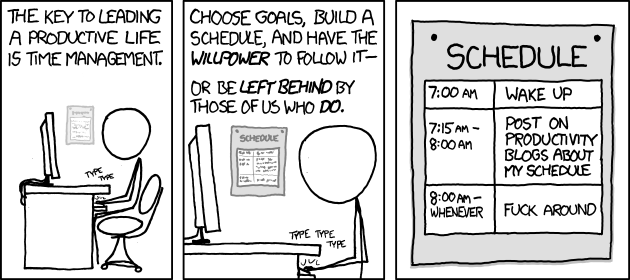
\includegraphics[scale=0.8]{comics/time_management.png}
\end{center}
\newpage
%%%%%%%%%%%%%%%%%%%%%%%%%%%%%%%%%%%%%%%%%%%%%%%%%%%%
% Formen
\subsubsection{Veranstaltungs- und Prüfungsformen}
Im folgenden werden wir verschiedene Veranstaltungs- und Prüfungsformen, die dir während deines Studiums über den Weg laufen können, kurz vorstellen, damit du dich darauf einstellen kannst, was alles auf dich zukommen kann. Die unten aufgezählten weiteren Kriterien können euch bei den Modulprüfungen begegnen. In jedem Fall müssen die genauen Kriterien für die zu erbringenden Leistungen spätestens in der ersten Veranstaltungswoche von dem Professor bekanntgeben werden, der die Veranstaltung hält.


\paragraph{Protokolle} In den Praktika musst du meistens wöchentlich eine oder ein paar Aufgaben lösen und diese sehr ordentlich und ausführlich protokollieren. Nur wer alle (oder fast alle – je nachdem) Versuchsprotokolle mit einem „ok“ gekennzeichnet bekommen hat, bekommt einen Praktikumsschein. Es kann aber auch möglich sein, dass zusätzlich noch mehr verlangt wird: Das Bestehen einer Klausur, das Teilnehmen an einem Seminar. Der Phantasie sind da kaum Grenzen gesetzt.


\paragraph{Hausarbeit} Hausarbeiten sind in der Informatik unüblich, in anderen Fächern wie zum Beispiel Pädagogik oder Politologie in Seminaren aber aufgrund der hohen Teilnehmerzahlen durchaus gebräuchlich. Eine Hausarbeit kannst du dir als einen mittelgroßen Aufsatz vorstellen, der nicht mit einem mündlichen Vortrag oder Referat verbunden ist. Und was „mittelgroß“ bedeutet, hängt unter anderem davon ab, wie lang oder wie kurz du ein bestimmtes Thema bearbeiten kannst. Im Zweifelsfall wird dir aber dein Veranstalter einen Tipp geben.


\paragraph{Referat} Referate sind in der Informatik ebenfalls unüblich, hier musst du in der Regel einen kurzen Vortrag über ein bestimmtes Thema halten, manchmal ist zusätzlich eine schriftliche Zusammenfassung zu leisten.


\paragraph{Seminar} Hier ist in der Regel eine schriftliche Ausarbeitung und ein Vortrag (mit anschließender Diskussion) zu einem bestimmten Thema zu leisten. Der Aufwand sollte nicht unterschätzt werden, da je nach Thema einiges an Literatur recherchiert und durchgearbeitet werden muss.

\paragraph{Vorlesung} Hier trägt der Veranstalter zu einem bestimmten Thema vor, dass dann auch in Übungen, falls angeboten, vertieft wird. Du kannst dir Vorlesungen als Frontalunterricht vorstellen, bei dem du zuhören darfst und solltest. Wenn du Glück hast, darfst du sogar ab und zu eine Frage stellen. Ganz engagierte Dozenten stellen sogar ab und zu eine Frage an die Hörer, um sicherzustellen, dass sie ihm auch gedanklich folgen. Vorlesungen an der Universität verlaufen aber oft sehr viel schneller als die Kurse in der Schule. Das heißt: \textbf{Passt du heute nicht auf, weißt du morgen schon nicht mehr, worum es überhaupt geht,} und aufzupassen fällt dir immer schwerer, und übermorgen gehst du vor lauter Frust schon gar nicht mehr hin. Die Übungszettel sind eine Möglichkeit für dich, sich mit dem Stoff der Vorlesung nochmal auseinanderzusetzen. Immerhin bist du nicht gezwungen, die Aufgaben allein zu lösen, sondern du darfst dich mit deiner Lerngruppe an die Zettel setzen, und mit mehreren Leuten hat man ja oft auch mehr Ideen. 


\paragraph{Mündliche Prüfung, „Fachgespräch“} Mündliche Fachgespräche werden oft in Vorlesungen Angeboten, wenn zu erwarten ist, dass sich nicht allzu viele Studis prüfen lassen werden. Ein 
solches Gespräch soll 20 bis 40 Minuten dauern. Am besten, du schaust dir vorher mal Prüfungsprotokolle an (beispielsweise auf der Homepage der Fachschaft angeboten), damit du einen Eindruck vom Prüfungsstil und den Lieblingsfragen des Prüfers bekommst.


\paragraph{Klausur} Eine Klausur ist in vielen Basismodulen vorgesehen. Sie dauert zwei bis vier Stunden, zum Bestehen musst du einen bestimmten Anteil der möglichen Punkte auch wirklich erreichen. Meistens liegt dieser Anteil so grob bei 50 \%, es kann je nach Fach und Schwierigkeit des Stoffs aber auch weniger sein!


\paragraph{Übungen} Jede Woche bekommst du einen Zettel mit Aufgaben, die du bis zur folgenden Woche lösen sollst. In den  „Tutorien“ oder „Übungen“ werden sie dann besprochen (dazu weiter unten noch mehr). Übungen sind etwas anders als Hausaufgaben. Einerseits solltest du sie zu Hause lösen. Andererseits bekommst du aber auch keine 6 eingetragen, wenn du sie nicht machst. Du musst dir noch nicht einmal eine gute Ausrede einfallen lassen.

Oft werden die letzten beiden Kriterien, Klausur und Übungen, kombiniert: Es gibt Übungsaufgaben, und die Punkte, die du damit erreichst, werden schon für die Klausur angerechnet; oder sie dienen dir nur zu deiner Vorbereitung auf die Klausur.


\paragraph{Tutoriumsleitung} Im Bachelor-Studiengang ist es möglich, durch das Leiten eines Tutoriums das Ergänzungsmodul zu komplettieren. Dadurch hast du nicht nur die Möglichkeit, das Institut für Informatik direkt zu unterstützen, sondern kannst außerdem noch wertvolle Erfahrungen im Bereich der Soft Skills sammeln.


\paragraph{Tutorien} Und wie ist das mit den Tutorien? Einmal in der Woche findet eine Veranstaltung bei eurem Tutor statt. Das ist auch ein Studi, der mit seinem Studium schon weiter ist und sich jetzt bereit erklärt hat, euch ein wenig beim Studieren zu helfen. Während eines solchen Tutoriums werdet ihr die Übungsaufgaben besprechen; meistens wird einer von euch eine Aufgabe vorrechnen. Das hat nichts damit zu tun, euch „vorführen“ zu wollen. Es sind aber zwei verschiedene Dinge, eine Lösung auf einen Zettel zu malen und eine Lösung anderen laut und mündlich, mit Hilfe einer Tafel, zu erklären. Die Möglichkeit, das zu üben, solltet ihr euch nicht entgehen lassen; ihr profitiert davon nicht nur für Seminarvorträge! Auch wenn ihr von eurem Tutor Punkte auf eure Lösungsversuche bekommt (oder viel zu oft nicht bekommt), ist es für euch keine Schande zuzugeben, dass ihr etwas nicht verstanden habt und euren Tutor danach zu fragen. Dafür sind Tutorien da!

Es ist wohl möglich, existierende Lösungen abzuschreiben und sich in den Tutorien wie eine Maus zu verkriechen und bloß nicht aufzufallen. Es haben auch schon Leute auf diese Weise einen Übungsschein (ohne Klausur) erhalten. Ihr wisst schon, gelernt will der Stoff trotzdem werden, denn in der mündlichen Prüfung gibt es kein Abschreiben und Verstecken.


Oft aber verlaufen Tutorien ganz anders. Der Tutor schreibt an und wirbelt herum, reißt sich ein Bein aus und redet sich ’nen Wolf, und alle Teilnehmer sitzen gelangweilt im Seminarraum, gucken an die Decke und bohren in der Nase. Was glaubt ihr, könnt ihr in einem solchen Tutorium lernen? Na? Wie sinnvoll und interessant und hilfreich ein Tutorium ist, ist zu einem großen Teil davon abhängig, wie die Teilnehmer es gestalten. Macht was draus!

\begin{flushright}Oliver und Sebastian\end{flushright}


	\begin{center}
		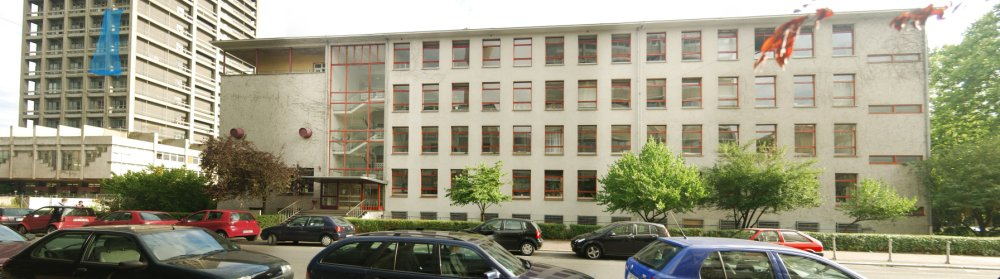
\includegraphics[scale=1.0]{bilder/rm_pano}
	\end{center}
\subsection{Sonstige Studiengänge}
	\subsubsection{Master Informatik}
	\spaltenanfang
Nachdem du es also gepackt hast, einen Bachelor mit einer Note von nicht schlechter als 3.0 zu erwerben, hast du dich für den Masterstudiengang an der Goethe-Universität Frankfurt entschieden.


Da die Ordnung für Studienanfänger im Masterstudiengang aber etwas verwirrend sein kann, gibt es dazu hier einige Erläuterungen.


Zunächst sollte bemerkt werden, das du dich entscheiden musst, was für einen Master du letztendlich machen willst, denn der Master in Informatik ist unterteilt in vier Schwerpunkte:
\begin{noindEnumerate}
\item Master mit Anwendungsfach
\item Master mit vertieftem Anwendungsfach
\item Master in allgemeiner Informatik
\item Master mit Spezialisierung
\end{noindEnumerate}

Hierzu sei gesagt, dass wenn du im Bachelor kein Anwendungsfach studiert hattest, du keine andere Möglichkeit hast, als den Master mit Anwendungsfach zu machen.


Hattest du hingegen im Bachelorstudium schon ein Anwendungsfach belegt, so kannst du nun ein neues Anwendungsfach belegen, das alte Anwendungsfach vertiefen oder dich zwischen dem Master in allgemeiner Informatik und dem Master mit Spezialisierung entscheiden, falls du dich gegen ein Anwendungsfach entscheidest.


Kommst du von einer anderen Universität und hast deinen Bachelor nicht an der Universität Frankfurt abgelegt, so kann es sein, das du Auflagen erteilt bekommst oder die Wahl des Schwerpunktes eingeschränkt wird. Die Vorlesungen, die du als Auflagen erteilt bekommst und die nicht mehr als 30 CP umfassen, musst du dann innerhalb von 14 Monaten erfolgreich abschließen.


Insgesamt geht das Masterstudium über vier Semester und besteht aus 120 CP. Egal für welche dieser vier Formen des Masterstudiums du dich entscheidest, am Ende musst du bei allen im Abschlussmodul eine Masterarbeit schreiben, die 30 CP bringt und gewöhnlich über ein Semester geht (6 Monate).


Die Informatikmodule sind in drei Gebiete aufgeteilt: „Informatik der Systeme“, „Grundlagen der Informatik“ und „Angewandte Informatik“. Je nach gewähltem Schwerpunkt musst du aus jedem der Gebiete eine bestimmte Anzahl an CP erbringen. Unter den Informatikmodulen muss jedoch mindestens ein Seminar und ein Praktikum sein.


Zusätzlich sind in jedem Schwerpunkt Ergänzungsmodule zu belegen, die 3 bis 6~CP bringen. Bei diesem Ergänzungsmodul handelt es sich um Veranstaltungen wie „Tutoriumsleitung“, die Vorlesungen „IT-Projektmanagement“ und „Neue Medien und Gesellschaft“. Desweiteren gehört das Modul „Soft Skills“ noch zu den Ergänzungsmodulen. In diesem Modul können im entsprechenden Umfang Veranstaltungen gewählt werden, die wissenschaftliches Arbeiten, Präsentationstechniken, Themen aus dem Bereich „Informatik und Gesellschaft“ und Wissensethik und weitere Soft Skills vermitteln. Diese Veranstaltungen werden nicht unbedingt vom Institut für Informatik angeboten, sondern auch z.B. vom Didaktischen Zentrum der Uni. 
\spaltenende

	\subsubsection{Bioinformatik}
    In Frankfurt hat man auch die M\"oglichkeit, Bioinformatik zu studieren und seinen Bachelor und Master darin zu machen.

Da es un\"uberraschend \"Uberschneidungen in den Studieng\"angen geben wird, werdet ihr fr\"uher oder sp\"ater auch auf Bioinformatiker treffen, wenn ihr es nicht sogar vielleicht selbst studieren wollt.
Der Studiengang selbst kann aber nur im Wintersemester angefangen werden.

Neben den f\"ur Bioinformatik spezifischen Veranstaltungen und den Veranstaltungen aus der Biologie wird man 
als Informatiker Bioinformatiker vor allem in den Grundvorlesungen sehen:
Bioinformatiker m\"ussen die beiden Programmierungs Veranstaltungen PRG1 und
PRG2, aus der Theorie Diskrete Modellierung, Datenstrukturen, und
Algorithmentheorie und aus der Mathematik Analysis und Lineare Algebra, sowie
Mathe 2 oder Stochastik und Numerik belegen.

Obwohl die Bioinformatik eigentlich Teil des Instituts f\"ur Informatik sind,
hat sich 2013 eine eigene Fachschaftsgruppe gebiltet, vor allem um Studenten am
Riedberg auch helfen zu k\"onnen.
	
	\subsubsection{Wirtschaftsinformatik}
    Wer lieber was mit Computern und Geld macht, kann sich im Anschluss an den Bachelor Informatik f\"ur den Master Wirtschaftsinformatik bewerben. Da sollte man aber schon gut gewesen sein, da der Studiengang stark zulassungsbeschr\"ankt ist.

Wer sich aber davon nicht abschrecken l\"asst, kann vom \glqq{ }Wirtschaftsstandort Frankfurt\texttrademark{ }profitieren\texttrademark\grqq{}.
Vorher BWL als Anwendungsfach geh\"ort zu haben lohnt sich dabei, da man bessere Chancen in den Studiengang reinzukommen hat,
je mehr man von den Grundlagen schon bescheinigt bekommen hat.
\\
    \begin{center}
        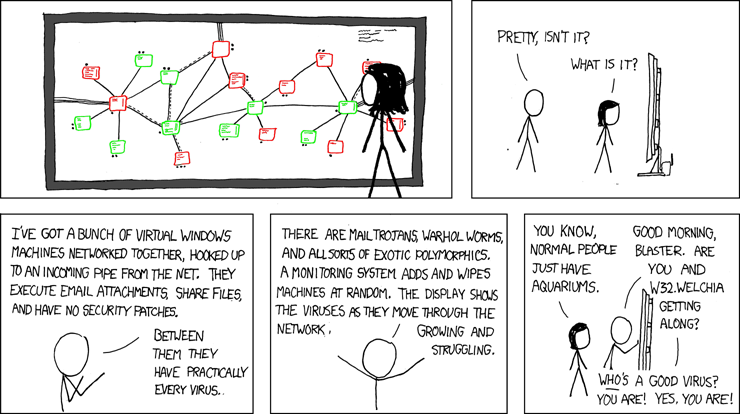
\includegraphics[width=\textwidth]{comics/network.png}
    \end{center}
\newpage
	\subsubsection{Informatik L3}
	\spaltenanfang
Seit dem Wintersemester 1997/98 kann man in Frankfurt Informatik auf Lehramt im L3-Studiengang (Gymnasiales Lehramt) studieren, seit dem Wintersemester 2010/11 zudem auch im L2-Studiengang (Haupt- und Realschullehramt) und im L5-Studiengang (Förderschule)  – mit sehr guten Berufsaussichten, denn viele entschließen sich nicht dazu und viele hören schon bald wieder auf.
Warum eigentlich? So ein Info-Lehramtsstudium ist doch ganz einfach.

Zunächst einmal stellen wir die für das Lehramtsstudium relevanten Ämter vor:

LA - \textit{Die hessische Lehrkräfteakademie}

Die hessische Lehrkräfteakademie (LA) (ehemals: LSA /Landesschulamt, und davor AfL / Amt für Lehrerbildung).
Die LA ist dem Hessischen Kultusministerium direkt untergeordnet und ist verantwortlich für die Ausbildung von Lehrkräften aller Fachrichtungen und Schulformen in ganz Hessen.
Du wirst im Regelfall mit der LA direkt nur max. dreimal zu tun haben: Bei deinem „Orientierungspraktikum“ und bei deinem „Betriebspraktikum“ und deinem 1. Staatsexamen.
Kontakt mit der LA kannst du am besten aufnehmen, indem du an den zuständigen Sachbearbeiter eine E-Mail schickst oder anrufst.


SPS-Büro \textit{Büro für Schulpraktische Studien}

Das SPS-Büro der ABL (Akademie für Bildungsforschung und Lehrerbildung) übernimmt innerhalb der Goethe-Universität die Koordination der Schulpraktischen Studien (SPS), auch hierzu später mehr. Du findest das SPS-Büro momentan im Juridicum auf dem Campus Bockenheim im 10. OG.
Du meldest dich beim SPS-Büro für die Schulpraktischen Studien an und im Gegensatz zu allen anderen Ämtern an der Universität muss dem SPS-Büro eine Änderung deines Studiums explizit (schriftlich) mitgeteilt werden (z.B.: bei einem Fachwechsel). Die Anmeldefristen für die SPS findest du auf der Homepage des SPS-Büros (www.abl.uni-frankfurt.de/40729270/Schulpraktische-Studien ). Diese Fristen sind absolut verbindlich und es gibt keinen Spielraum – also hier besonders genau sein!


ZPL – \textit{Zentrales Prüfungsamt für Lehramtsstudiengänge}
Das ZPL befindet sich momentan am Campus Bockenheim im 10 Stock Juridicum. Es ist dafür verantwortlich, die von dir abgelegten Prüfungen (abgeschlossene Module) zu registrieren und die Zwischenprüfung, sowie die Meldung zur ersten Staatsprüfung zu verwalten.
Zu Beginn deines Studiums meldest du dich zur Zwischenprüfung beim ZPL an (Informationen bekommst du entweder auf der Homepage des ZPL, oder bei einer Einführungsveranstaltung). Du legst die Zwischenprüfung automatisch ab, wenn du in vollständig abgeschlossenen Modulen insgesamt 90 CP beim ZPL in Form von kopierten (!) Modulscheinen eingereicht hast - bei L2 brauchst du sogar nur 60 CP.
Die Zwischenprüfung kannst du ablegen, sobald du die benötigten CP gesammelt hast (hierbei gibt es genauere Auflagen, die du der Studienordnung entnehmen kannst), sie sollte allerdings spätestens zwei Semester vor der Meldung zur Ersten Staatsprüfung eingereicht werden, damit eventuelle formale Probleme behoben werden können.
Die Bescheinigung über ein ordnungsgemäßes Studium am Ende bekommst du übrigends genauso. Du reichst alle deine kopierten (!) Modulscheinen ein. Auch das solltest du mindestens ein Semester vor der Meldung zur Ersten Staatsprüfung machen.\\

Neben diesen Ämtern möchten wir dir einige Informationen zu einigen wichtigen Begriffen und Punkten im Lehramtsstudium geben.

\paragraph{Die Schulpraktischen Studien (SPS)}
Die SPS sind der praktische Teil der universitären Lehramtsbildung. Du wirst im Studiengang L2 bzw. L5 in deinem Studium zwei SPS-Veranstaltungen absolvieren, eine bildungswissenschaftliche und eine fachwissenschaftliche. Die SPS setzen sich in dem Fall aus einem Vorbereitungsseminar in einem Semester, einem 5- wöchigen Schulpraktikum in den Semesterferien und einer Nachbereitungsveranstaltung im folgenden Semester zusammen.
L3 Studierende fallen in die Praxissemesterregelung. Ihr habt nur ein Praktikum das über ein Semester geht. Mehr erfahrt ihr unter:http://www.abl.uni-frankfurt.de/51930903/Praxissemester-L3

\paragraph{Modulscheine}
Im Gegensatz zu den meisten anderen Studiengängen ist das Lehramtsstudium noch nicht vollständig digitalisiert. Du kannst dir auf der Seite des ZPL sog. „Modulscheine“ ausdrucken, in welche die Dozenten die Prüfungsnoten eintragen müssen.
In der Regel ist es so, dass zu einem Modul mehrere Veranstaltungen gehören, in diesem Fall ist es empfehlenswert in der zweiten Veranstaltung nur eine Kopie des bereits zum Teil ausgefüllten Scheins abzugeben, denn ein Verlust ist für dich mit erheblicher Arbeit verbunden.

\paragraph{Die fachspezifischen Anhänge und die Studienordnung}
Die Studienordnung für Lehramtsstudiengänge setzt sich aus der
"Studienordnung" und den "fachspezifischen Anhängen" zusammen. Die Studienordnung regelt generelle Formalia, wie zum Beispiel den Umfang des Studiums, die benötigten CP und die Abläufe der Ersten Staatsprüfung und der Zwischenprüfung.
Die fachspezifischen Anhänge hingegen beschränken sich auf ein Fach (z.B.: L3 Informatik) und beinhalten eine Übersicht über die zu belegenden Module.
Sowohl die Studienordnung, als auch die fachspezifischen Anhänge finden sich auf der Homepage der ABL und sind leicht über eine Suchmaschine unter dem Stichwort "fachspezifische Anhänge Uni Frankfurt" zu finden.
\textbf{Zu Beginn des Studiums empfiehlt sich auf jeden Fall eine Lektüre der Studienordnung sowie der fachspezifischen Anhänge.}
Innerhalb der fachspezifischen Anhänge findest du einen Studienverlaufsplan, also einen exemplarischen Plan, in welcher Reihenfolge und in welchem Semester du welche Veranstaltungen belegen kannst. Die Vorgaben sind allerdings nicht verpflichtend, manchmal muss aber auf die Reihenfolge geachtet werden.

\paragraph{Orientierungspraktikum (OP) (betrifft nicht L3-Erstis)}
Das OP muss durch das LA bestätigt worden sein, bevor du dich für die ersten SPS anmelden kannst. Es muss in einer pädagogischen Institution stattfinden und 4 Wochen (120 Stunden) dauern. Auf der Homepage des LA befindet sich ein Vordruck für einen Praktikumsbericht, der ausgefüllt werden muss. Auf der letzten Seite des Berichts ist ein Formular das von dir und vom Betrieb auszufüllen ist, zudem muss vom Betrieb eine (informelle) Bestätigung ausgestellt werden.
Für das OP können Tätigkeiten aus FSJ oder ähnlichem anerkannt werden, in diesem Fall muss nur eine Bescheinigung des Betriebs beiliegen sowie die letzte Seite ausgefüllt werden. Der Bericht entfällt in diesem Fall.
Zu beachten: Ihr könnt euch nichts anrechnen lassen was ihr in eurer Schulzeit gemacht habt.

\paragraph{Betriebspraktikum (BP) (betrifft nicht L3-Erstis)}
Das Betriebspraktikum umfasst 8 Wochen bei "branchenüblicher Arbeitszeit" (in Ordnung sind auch zwei mal 4 Wochen, auch in unterschiedlichen Betrieben). Es muss in einem Betrieb stattfinden, der nichts mit (pädagogisch-) sozialen Tätigkeiten zu tun hat. Auch hierzu findest du auf der Homepage des LA einen Vordruck für einen Praktikumsbericht. Es wird eine Bestätigung des Betriebs benötigt.
Als Betriebspraktikum können Nebenjobs in nicht-pädagogischen Betrieben anerkannt werden, die über einen längeren Zeitpunkt gemacht wurden. In diesem Fall benötigst du eine Bestätigung des Betriebs und musst den Bericht dennoch schreiben!
Das Betriebspraktikum muss vor der Meldung zur Ersten Staatsprüfung eingereicht werden.
\spaltenende

\newpage

%\subsection{Bachelor-/Masterordnung}

%\subsection{Teilzeitstudium}
	
\newpage
\section{Die Uni}
	\subsection{Wo ist was?}
			\begin{center}
			\texttt{ It's dangerous to go alone! Take this. }
			\fbox{
			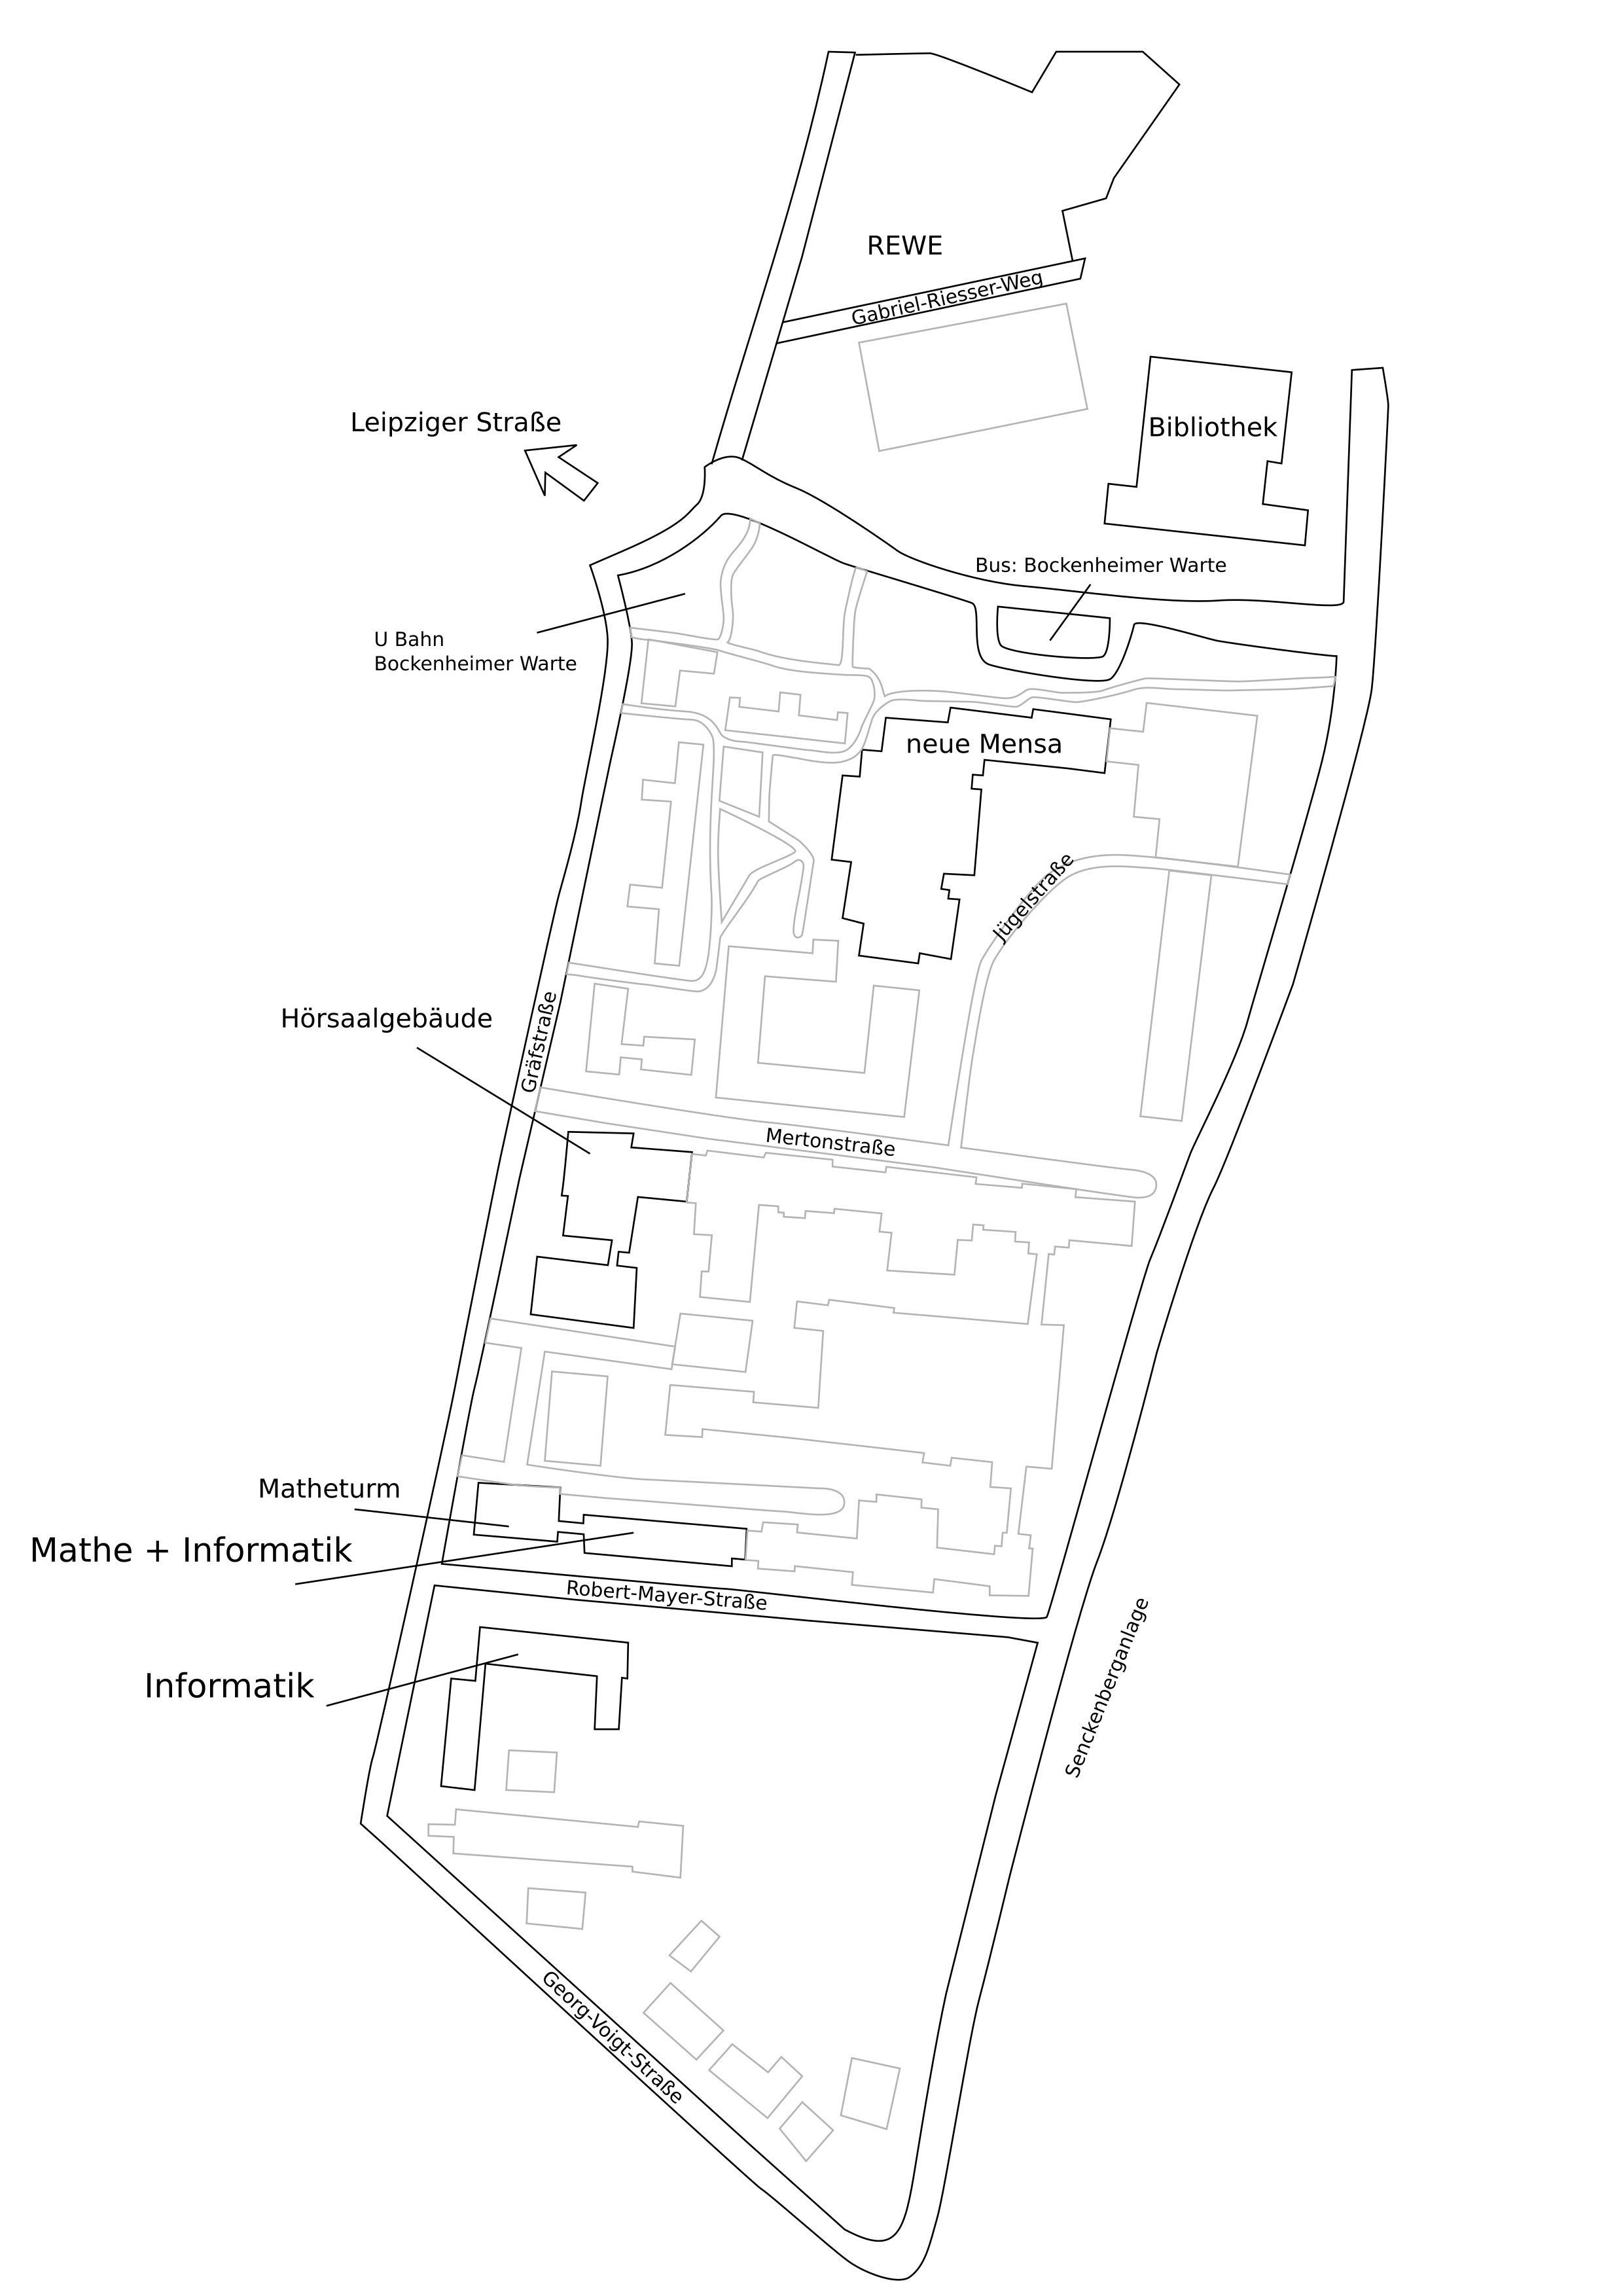
\includegraphics[width=0.8\linewidth]{bilder/KarteB}}
            \\Bockenheim Map
			\end{center}
		\pagebreak
    		\subsubsection{Bockenheim}
			Wichtig für die Vorlesungen und Übungen:\\
			\fbox{
			\begin{tabular}{rrl}
				Hörsäle: & H 1 - H 16  & Teil des Hörsaalgebäudes über dem Cafe.\\
				{} & H I - H VI  & Andere Teil des Hörsaalgebäudes, welcher nicht\\
				{} & {} & über dem Cafe ist.\\
				{} & Magnushörsaal & In der Informatik\\
				{} & {} & {}\\
				Seminarräume: & SR9, SR11 & Informatik EG\\
				{} & 307 & Informatik 3.Stock\\
				{} & NM...& Diese Räume sind in der neuen Mensa\\
				{} & \multicolumn{2}{l}{Alle anderen dreistellingen Zahlen sind im Matheturm}\\
			\end{tabular}}
			\ \\\\ 
			Sonstige Interessante Orte:\\
			\fbox{
				\begin{tabular}{rp{11cm}}
					Cafe Struwwelpeter: & Hier gib es Getränke und kaltes Essen. Du findest es im\\
					{} & Hörsaalgebäude.\\
					Cafeteria: & Verkauft warme Gerichte und gehört zum Studentwerk.  \\
					{} & Ihr findet die Cafeteria in der neuen Mensa.\\
					Leipziger Straße: & Falls ihr aus gegebenen Anlässen keine Lust mehr auf Mensa essen habt, dann gibt es hier alles was das Herz begehrt(Nicht nur Essen).
				\end{tabular}
			}
		
		\subsubsection{Westend}
			Das Westend ist für euer Studium erst interessant, wenn ihr ein Anwendungsfach der Geisteswissenschaften gewählt habt oder ihr Fragen oder Probleme mit dem HRZ oder der Uni habt. Außerdem ist das Westend ein perfekter Ort für eine Studentensafari. Nirgendwo sonst gibt es einen Lebensraum, wo die Reviere so unterschiedlicher Studenten aufeinander treffen. \\
		
		\subsubsection{Riedberg}
			Genauso wie das Westend, ist der Riedberg erst mit der Wahl eines Anwendungsfaches interessant. Bis auf der Tatsache, dass wir uns von Anfang an dort wohlfühlen.
		\subsubsection{Niederrad und Ginnheim}
			Orte, wo die meisten von uns nie sein werden. In Ginnheim befinden sich die Unisportanlagen und in Niederrad die Medizin.
	


		
	\newpage
    \subsection{Goethe-Card + Semesterticket}
    \begin{wrapfigure}[8]{r}{0.48\textwidth}
     \vspace{-5mm}
  \begin{center}
     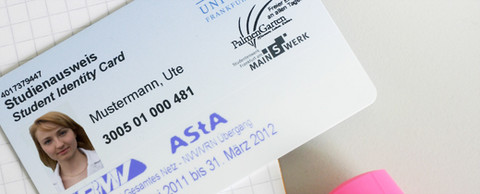
\includegraphics[scale=0.5]{bilder/goethecard}
  \end{center}
\end{wrapfigure}

Nach der erfolgreichen Immatrikulation an unserer Universität bekommst du im Studien-Service-Center eine schicke Chipkarte mit deinem Foto und einigen bildhaften Logos und Beschriftungen drauf. Möglicherweise erfährst du auch gleich, dass sie \emph{Goethe-Card} heißt und als Studienausweis dient. Warum braucht man überhaupt so etwas, wenn man bereits einen ordinären Ausweis hat?

Der wichtigste Grund ist die Tatsache, dass man damit sofort feststellen kann, ob du zum aktuellen Zeitpunkt an der Goethe-Universität studierst: In diesem Fall wurde das blau aufgetragene Gültigkeitsdatum unten zu diesem Zeitpunkt noch nicht überschritten. 

Falls du jetzt ein Blick auf deinen Studienausweis wirfst, wirst du bemerken, dass dort als Enddatum der letzte Tag des laufenden Semesters steht. Daher wirst du, solange du bei uns bleibst, einmal alle 6 Monate diesen Eintrag updaten müssen. Das geht über einen der mehreren extra dafür erstellten und überall auf dem Uni-Gebiet platzierten Automaten, die oft auch \emph{Validierer} genannt werden. Sollte man sein Studium absolviert oder abgebrochen haben, wird der Validierer das Enddatum der Gültigkeit nicht ändern.

Auf der Goethe-Card sind außerdem dein Foto, dein Name und auch deine persönliche Identifikationsnummer (\emph{Matrikelnummer}) in der Universität aufgeschrieben\footnote{Deine Matrikelnummer ist 7-stellig und entspricht den letzten 7 Ziffern der 12\hbox{-}stelligen Zahl auf dem Goethe-Card.}. Diese Angaben helfen nicht nur den Profs, dich eindeutig zu identifizieren, sondern auch dir, deine während der Prüfung vergessene Matrikelnummer schnell zu finden.

Aber das ist noch nicht alles, was du mit der Goethe-Card machen kannst:

\begin{itemize}
	\item Du kannst darauf mittels spezieller Geldautomaten-ähnlichen Geräten darauf \textbf{Geld aufladen}, um damit in der Mensa für das Essen oder auch in der Uni-Bibliothek für die Verwendung des Kopierers zu bezahlen
	\item Du kannst sie als einen \textbf{digitalen Schlüssel} für die super modernen Schließfächer am Campus Westend verwenden
	\item Du kannst damit \textbf{kostenlos} den \textbf{Palmengarten} besuchen
	\item Du kannst damit\textbf{ Bücher in der Uni-Bibliothek ausleihen}
\end{itemize}

Und - last but not least - du kannst damit \textbf{kostenlos} in allen öffentlichen Verkehrsmitteln außer ICE, IC und EC in Hessen fahren! Vor dem 01.03.2013 war das NVV-Gebiet leider nicht mit dabei, daher solltest du deine Goethe-Card unbedingt updaten, wenn du diese vor diesem Tag erhalten hast und kein Logo von NVV neben dem Logo von RMV siehst.

Allerdings pass auf: Außerhalb von Hessen funktioniert das nicht mehr! Auf der nächsten Seite findest du eine Karte mit dem skizzierten Geltungsbereich des Semestertickets.

Ausserdem: Der Verlust der Goethe-Card kann recht schmerzlich sein - z.Z. liegt die Gebühr bei Verlust und darauf folgende Neubeantragung (Campus Westend) bei 50 Euro.

Weitere Informationen zur Goethe-Card kannst du bei Interesse hier finden:\\
\url{http://www.rz.uni-frankfurt.de/44160530/Goethe-Card}
\begin{flushright}Pavel, korrigiert von Sabrina \end{flushright}
    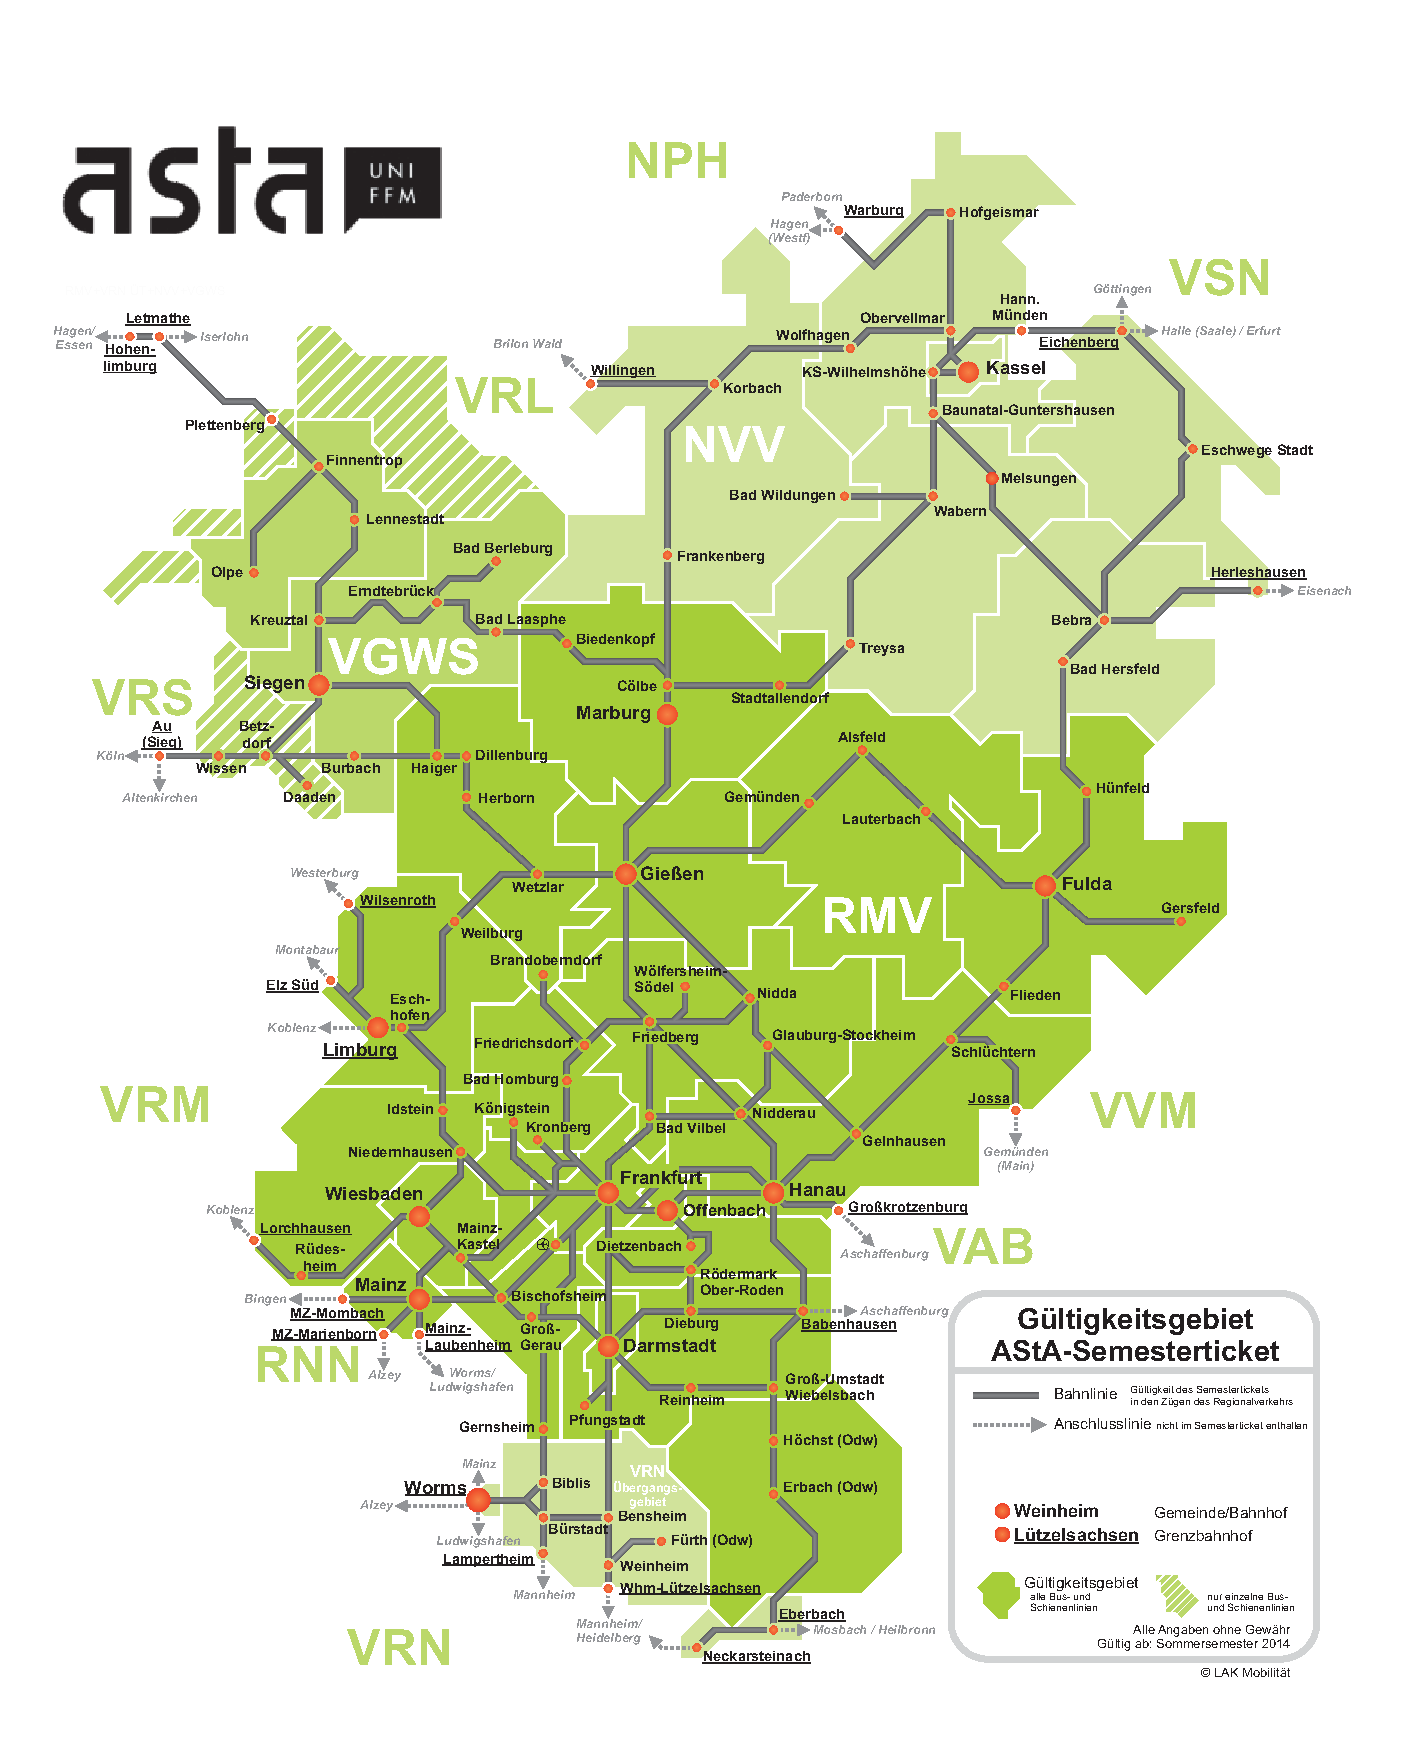
\includepdf{tabellen/semesterticket}

    \subsection{Services und Einrichtungen}
    \subsubsection{Internet}
    Ach ja, das Internet von dem alle immer reden...\\

\spaltenanfang
Eigentlich sollte ja alles ganz einfach sein.
Die Uni war schon am Internet, bevor es das WWW gab und sollte deshalb mehr Erfahrung als der Rest der Welt haben.
Aber was stattdessen passiert ist, ist dass das Netz an der Uni gewachsen ist
und inzwischen die Komplexit\"at eines Lebewesens gepaart mit der
Zuverl\"assigkeit eines Informatikstudentens morgens um 08:00 s.t. erreicht
hat. Besonders in der Informatik, wo jeder einen eigen Webserver betreiben
kann, betreibt jeder einen eigenen Webserver. Das Resultat ist eine
uneinheitliche Mischung, in der jede Veranstaltung eigene Rituale hat,
\"Ubungsanmeldungen \"uber das Internet abzuwicklen oder die Folien der
Vorlesung zu ver\"offentlichen. Au{\ss}erdem ist die Netzwerkinfrastruktur
uneinheitlich und die unterschiedlichen WLAN SSIDs, mit denen man sich
verbinden kann, kommen einem wie ein Dschungel aus elektromagnetischer
Strahlung vor. Sich dann noch Passworte f\"ur Vorlesungen, unterschiedliche
Uni-Mailadressen und all die verschiedenen Accounts zu merken, macht die
Verwirrung komplett.  Und damit wurde das Internet zu dem, was es heute ist:
\textbf{Dem ersten Endgegner der Informatik}.

\textbf{Eure Accounts:}
Grunds\"atzlich bekommt jeder Student an der Uni Frankfurt einen Account vom \textbf{HRZ}, dem \textit{Hochschul RechenZentrum}\footnote{\url{http://www.rz.uni-frankfurt.de}}.
\"Uber diesen Account k\"onnt ihr euch zu Klausuren und Veranstaltungen anmelden, eure Studiendaten abfragen, E-Mails schreiben und lesen und habt einen WLAN-Zugriff \"uberall da an der Uni, wo WLAN grade funktioniert. Als eingeschriebene Studenten habt ihr eure Zugangsdaten und eine TAN Liste zugeschickt bekommen. 

Aber als Informatiker habt ihr auch die M\"oglichkeit, euch einen Account im speziellen Informatikrechenzentrum, dem \textbf{RBI} (\textit{RechnerBetrieb Informatik})\footnote{\url{http://www.rbi.cs.uni-frankfurt.de}} anlegen zu lassen. Da k\"onnt ihr auch E-Mails benutzen, Windows- und Softwareentwicklungs Lizenzen bekommen und k\"onnt sogar bis zu 500 Seiten im Semester kostenlos drucken. Au{\ss}erdem stehen in der Informatik Computer, die ihr nur mit einem RBI-Account benutzen k\"onnt. Wer beim Vorkurs war, kennt das ja schon.

F\"ur manche Veranstaltungen bekommt ihr eventuell noch extra Accounts. Zum Beispiel, wenn ihr Hochleistungscomputer programmieren sollt, kann euch der Veranstalter erlauben, mit seinem Spielzeug zu spielen und gibt euch extra Accounts. Aber normalerweise braucht ihr erstmal nur die beiden Zug\"ange der beiden oben genannten Rechenzentren.

\textbf{WLAN:}
Sich an der Uni mit dem WLAN zu verbinden, ist im Prinzip einfach.
Trotzdem sollte man vorher alle Rituale, die g\"ottliches Wohlwollen hervorrufen, mit h\"ochster Sorgfalt abhalten,
denn die WLAN Ausleuchtung der Uni ist nicht \"uberall gew\"ahrleistet.

Es gibt uniweit drei unterschiedliche Netze.\\
\textbf{FREIFLUG} ist das langsamste (und unsicherste) Netzwerk, aber daf\"ur kommt man auch fast immer rein. Dazu wirst du erst auf eine interne Uniseite umgeleitet und musst dich da mit deinen HRZ-Daten anmelden, bevor du ins Internet kommst. Das ist dann unversch\"usselt, was in der Informatik nicht zu emfehlen ist.\\
FLUGHAFEN ist ein verschl\"usseltes uniweites Netzwerk, aber nicht so gut wie:\\
\textbf{eduroam} ist ein Netwerk, mit dem du als Student sogar an vielen anderen Universit\"aten weltweit ins Internet kommst (Achtung, damit dies auch weltweit funktioniert, muss der Login wie folgt sein: \textit{<deinHrzAccountName>@uni-frankfurt.de} - auch wenn Du diese Email-Adresse nicht hast!).
Es ist ein 802.1x Netz f\"ur das du aber vorher ein Zertifikat\footnote{\url{https://www.pki.dfn.de/fileadmin/PKI/zertifikate/deutsche-telekom-root-ca-2.der}} brauchst (ist auf machen Systemen (auch mobil) schon vorinstalliert).\\
Schlie{\ss}lich gibt es noch WLAN-RBI-VPN von der RBI, mit dem du dich \"uber OpenVPN verbinden kannst.

Wie du dich genau mit dem WLAN verbindest kannst du auf den Seiten des jeweiligen Rechenzentrums nachlesen und ist von deinem Betriebssystem abh\"angig. Aber wer braucht als Informatiker schon Internet, Papier und Bleistifte sind wichtiger als Computer.






\spaltenende

    \subsubsection{Softwarelizenzen}
    \subsubsection{Bücherreien}
	\subsubsection{QIS/LSF und dessen Funktion}
	%\subsection{Aufbau der Unipolitik}
\newpage
\section{Die Informatik}
	\subsection{Robocup-AG}
    \spaltenanfang
Wir schreiben das Jahr 2050. Im Madison Cube Garden stehen sich 11 menschliche und 10 Roboter-Fußballer gegenüber. Moment, 10? Da fehlt doch einer! Aha, Bender steht rauchend und trinkend auf der VIP-Tribüne und klaut Schmuck und Uhren!
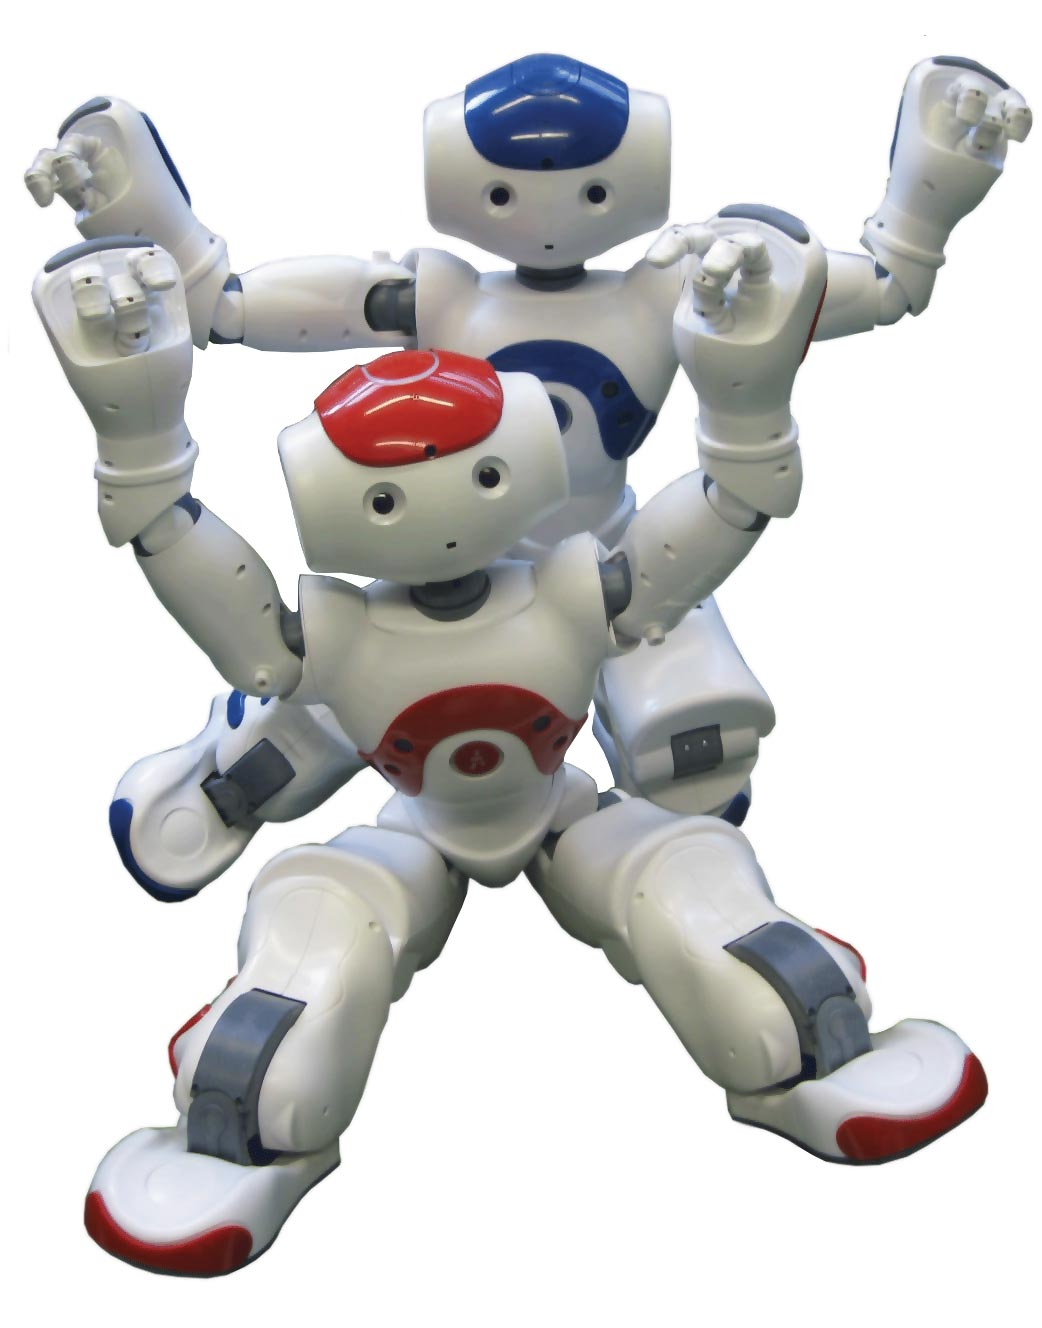
\includegraphics[width=8cm]{bilder/robocup1}

So oder ähnlich oder komplett anders könnte die Zukunft aussehen, wenn DU bei unserem Team mitmachst!

Doch blicken wir zurück ins Jahr 2009, wo alles seinen Anfang fand. Mittlerweile hat schon fast jede Erd-Universität eigene Prototypen, unter anderem auch die Robocup-AG der Universität Frankfurt. Die Vorform von Bender, Nao genannt, hat noch bessere Manieren und sieht relativ harmlos aus, ist aber leider auch noch ziemlich unfähig. Und hier kommt das Team Bembelbots ins Spiel, die Studenten der Robocup-AG, die ihm Leben einhauchen. Unter der Schirmherrschaft des Joint Robotics Lab (JRL) arbeiten wir ständig an der Verbesserung von Naos Fähigkeiten.

Unabhängig vom Kenntnisstand findet sich bei uns für jeden eine Aufgabe, der Robocup bietet für jeden Teilbereich der Informatik spezielle Herausforderungen. So kann man sich entscheiden, ob man mit Hilfe von Bildverarbeitung, Bewegungsoptimierung, Künstlicher Intelligenz oder aber auf einem ganz anderen Weg unseren Robotern zum Erfolg verhilft.

Und mit etwas Glück erfüllen wir das oben aufgeführte Szenario von Professor Farnsworths ``Was wäre, wenn?''-Maschine und lassen unsere Roboter wirklich irgendwann gegen menschliche Gegner antreten. Wenn du interessiert bist, mitmachen oder einfach mal reingucken willst, bist du herzlich eingeladen, in der Robert-Mayer-Straße 8, Raum 09a (im Kellergeschoss) vorbeizukommen, oder du besuchst unsere Internetseite zum Robocup/JRL:
 
\url{http://www.bembelbots.de}

Hier findest du neben Infos zum Robocup auch andere studentische Projekte des Joint Robotics Lab. 
\spaltenende

\includegraphics[width=0.8\textwidth]{bilder/Bembelbots}


\label{fachschaftsarbeit}
\section{Die Fachschaft}
    
\subsection{Wer sind wir?}
    \glqq\textit{Wir befinden uns im Jahre \the\year{} n.Chr. Die ganze Informatik ist von der Faulheit besetzt... Die ganze Informatik? Nein! Ein von unbeugsamen Freiwilligen bevölkerter Raum hört nicht auf, dem Eindringling  Widerstand zu leisten.} \grqq

    Spaß beiseite. Wir sind die aktive Fachschaft der Informatik. Aktiv, weil alle Studenten Teil der Fachschaft sind. Die ist n\"amlich als alle Studenten eines Fachbereichs definiert.

    Nochmal, das hei{\ss}t, dass \emph{ihr alle Fachschaft seid}. Aber nur mache werden aktiv und machen was. %Und das sind wir.
    Grunds\"atzlich kann man \"uber uns sagen, dass wir ein versprengter Haufen von verrückten, abgedrehten Nerds, Geeks und anderer Lebensformen sind, deren Existenz in den Augen von Au{\ss}enstehenden schwer nachzuvollziehen ist.
    Aber das sind alles sowieso nur Vorurteile, die wir nicht von uns weisen. Welche davon stimmen und welche nicht, dürft ihr gerne selber herausfinden. Wir bezeichnen uns aber gerne als normal.



\subsection{Was machen wir?}
    Es wird gerne behauptet, der Sinn einer Informatik-Fachschaft sei, st\"andig zu trinken und Rollenspiele zu spielen.
    Da wir uns als Wissenschaftler vorurteilsfrei der Wahrheit verschrieben haben, m\"ussen wir sagen: ja, das stimmt teilweise.
    Gem\"utliches Beisammensein ist aber nur ein Teil unserer Arbeit.

    Der andere große Teil betrifft haupts\"achlich den Universit\"atsalltag.
    Studenten sind in viele Prozesse der Entscheidungsfindung an der Uni
    mit eingebunden.
    Zum Beispiel verbringen wir als studentische Vertreter viel Zeit in Kommissionen und mit Gremienarbeit.
    Die haben dann die unterschiedlichsten Namen und Aufgaben.
    Die habt ihr ja alle bei der W\"orterbuchattacke am Anfang mitbekommen.
    Aber unser inoffizielles OE-Motto ist ''Wir glauben an Wiederholungen!'' also frischen wir euren Cache im Kopf nochmal auf:
    \begin{itemize}
        \item I-Rat - die offizielle Ger\"uchtek\"uche
        \item FBR - wo man zusieht, dass keiner am Fachbereich Mist macht.
        \item LuSt-Ausschuss - weil's Spa{\ss} macht
        \item Prüfungsausschüsse - sind halt wichtig, und so.
        \item QSL-Mittelausschuss - Geld verteilen muss auch sein.
        \item FSR - das sind wir offiziell.
        \item FSK - und das sind wir und alle anderen Fachschaften.
    \end{itemize}
    Au{\ss}erdem sind wir daf\"ur da, dass wir anderen Studenten helfen. Dies kann auf unterschiedlichste Weise passieren:
    \begin{itemize}
        \item Bei Fragen zu organisatorischen Themen können wir selber Antworten geben oder auf Personen verweisen, die euch da besser weiterhelfen können.
        \item Falls ihr berechtigte Kritik an Vorlesungen und/oder Übungen nicht selbst äußern wollt oder diese ignoriert wird, sind wir dafür da, diese Kritik an die verantwortliche Person weiterzutragen, wozu uns mehr Möglichkeiten zur Verfügung stehen.
        \item Wir organisieren die Orientierungsveranstaltung für Erstsemestler, damit ihr in der ersten Woche nicht vor lauter ungewohnten Sachen erschlagen werdet.
        \item Wir erstellen dieses Heft, damit ihr wichtige Themen nachschlagen könnt.
        \item Wir organisieren Sommerfest und Weihnachtsfeier!
    \end{itemize}
    Im Prinzip machen wir also alles\dots\hspace{1cm} Zumindest was Studenten so tun.




\subsection{Du willst zu uns?}
    \glqq Wir grillen gerade und haben ein wenig zu trinken da. Willst du nicht zu uns stoßen?\grqq { }Bei vielen Fachschaftlern hat diese Masche schon funktioniert. Doch gerüchteweise gibt es unter den Studenten auch immer ein paar ''Rationalisten'' die ''Argumente'' brauchen. Und weil ''Wir sind cool!'' nicht immer ausreicht, sind hier ein paar Kommentare von und über uns:
    \begin{itemize}
        \item Wir sind cool!
        \item Social Engineering lernen, wo besser als an der Uni?
        \item Die Gerüchteküche sind wir.
        \item Form die Uni nach eurem Bild.
        \item Lern die Professoren kennen.
        \item Mach die Uni zu deinem Zuhause an der Uni.
        \item Lern die Studenten kennen, die dir dein Zweistundenproblem in zwei Minuten lösen.
        \item Werde Student, der die Zweistundenprobleme in zwei Minuten löst.
        \item CP für Gremienarbeit.
        \item Das Direktorat fragt dich!
        \item Entscheide, für wen Ausnahmen gemacht werden.
        \item Firmenpolitik begegnet dir überall. Lerne diese Kunst an der Uni.
        \item Fachschaftsfeiern.
    \end{itemize}
    Bleibt nur noch zu sagen, dass ihr keine besonderen F\"ahigkeiten braucht - die Fachschaft ist ja keine Castingshow.
    Manche von uns reden nicht gerne, andere k\"onnen nicht gut schreiben und sind dabei weder am Trinken noch am Grillen.
    Wie gesagt, wir sind halt nur die Leute, die an der Uni rumh\"angen, nur das wir uns auch f\"ur die Uni an sich interessieren.



	
	
\end{document}
